\documentclass[11pt,a4paper]{report}
\usepackage[a4paper,top=2.5cm,bottom=2.5cm,left=2.5cm,right=2.5cm]{geometry}
\usepackage{graphicx}
\usepackage{float}
\usepackage{tikz}
\usetikzlibrary{calc}
\usepackage{setspace}
\usepackage{booktabs}
\usepackage{multirow}
\usepackage{amsmath}
\usepackage{amssymb}
\usepackage{caption}
\usepackage{subcaption}
\usepackage[hidelinks]{hyperref}
\usepackage{fontspec}
\usepackage{polyglossia}
\setdefaultlanguage{vietnamese}
\setmainfont{Times New Roman}

\setstretch{1.15}
\setlength{\parskip}{6pt}
\setlength{\parindent}{0pt}
\newcommand{\figwidth}{0.85\textwidth}

\begin{document}

% ======================= TRANG BÌA ==========================
\begin{titlepage}
\thispagestyle{empty}
\centering
\begin{tikzpicture}[remember picture, overlay]
  \draw[line width=0.8pt]
    ($(current page.north west) + (2cm,-2cm)$)
    rectangle
    ($(current page.south east) + (-2cm,2cm)$);
\end{tikzpicture}

{\bfseries\large ĐẠI HỌC KHOA HỌC VÀ CÔNG NGHỆ HÀ NỘI\par}
\vspace{4pt}
{\bfseries\large KHOA CÔNG NGHỆ THÔNG TIN VÀ TRUYỀN THÔNG\par}

\vspace{2.4cm}
\IfFileExists{figures/logo.png}{
  
\includegraphics[width=6cm]{figures/logo.png}\par
}{
  \vspace*{3.5cm}
}
\vspace{1.8cm}

{\bfseries\Large BÁO CÁO KHÓA LUẬN TỐT NGHIỆP\par}
\vspace{10pt}
{\bfseries\Large Đánh giá So sánh các Mô hình Học sâu cho Bài toán Phân loại Tổn thương Da trên Tập dữ liệu Dermoscopy Công khai\par}

\vspace{2.0cm}
\begin{tabular}{@{}rl@{}}
\textbf{Sinh viên thực hiện:} & Nguyễn Trọng Bách -- 23BI14057\\[10pt]
\textbf{GVHD nội bộ:} & TS. Nghiêm Thị Phương\\[8pt]
\textbf{GVHD bên ngoài:} & TS. Vũ Trọng Sinh\\
\end{tabular}

\vfill
{\large Ngày 26 tháng 2 năm 2026\par}
\end{titlepage}

% ======================= LỜI CẢM ƠN ==========================
\chapter*{Lời cảm ơn}
\addcontentsline{toc}{chapter}{Lời cảm ơn}

Trước hết, tôi xin bày tỏ lòng biết ơn chân thành đến giảng viên hướng dẫn bên ngoài, TS.~Vũ Trọng Sinh, vì những chỉ dẫn vô giá, sự hỗ trợ liên tục và kiến thức sâu rộng của thầy. Những hiểu biết thực tiễn của thầy về hình ảnh y khoa đã đóng vai trò then chốt trong việc định hướng nghiên cứu này.

Tôi vô cùng biết ơn giảng viên hướng dẫn nội bộ, TS.~Nghiêm Thị Phương, vì sự động viên không ngừng, lòng kiên nhẫn và sự dẫn dắt học thuật trong suốt thời gian tôi học tại Đại học Khoa học và Công nghệ Hà Nội. Những phản hồi mang tính xây dựng của cô đã nâng cao đáng kể chất lượng của khóa luận này.

Lời cảm ơn chân thành gửi đến bạn gái tôi vì đã luôn bên cạnh trong những đêm dài gỡ lỗi và huấn luyện mô hình. Sự hỗ trợ tinh thần và thấu hiểu của bạn là nguồn động lực to lớn đối với tôi.

Cuối cùng, tôi muốn bày tỏ lòng biết ơn sâu sắc nhất đến gia đình. Gửi đến bố mẹ, con cảm ơn vì tình yêu vô điều kiện, những hy sinh và vì luôn tin vào tiềm năng của con. Con xin dành cột mốc này cho bố mẹ.

% ======================= TÓM TẮT ==========================
\chapter*{Tóm tắt}
\addcontentsline{toc}{chapter}{Tóm tắt}

Ung thư hắc tố (melanoma) chiếm phần lớn số ca tử vong do ung thư da, nhưng lại có tỷ lệ sống sót sau 5 năm trên 99\% nếu được phát hiện sớm. Để chuyển hóa thực tế lâm sàng này thành một công cụ tự động đòi hỏi không chỉ một mô hình có năng lực mà còn cần một quy trình huấn luyện có khả năng xử lý tình trạng mất cân bằng lớp nghiêm trọng vốn đặc trưng của các tập dữ liệu dermoscopy: trong bộ dữ liệu chuẩn ISIC 2018, lớp chiếm ưu thế Melanocytic Nevus vượt trội lớp hiếm nhất, Dermatofibroma, với tỷ lệ gần 60:1.

Khóa luận này đánh giá bốn kiến trúc học sâu --- EfficientNet-B0, ResNet50, DenseNet121 và Swin-Tiny --- trong cùng một pipeline huấn luyện được thiết kế để đối phó với sự mất cân bằng đó. Pipeline kết hợp Lấy mẫu Ngẫu nhiên có Trọng số, tăng cường dữ liệu Mixup và CutMix, làm mượt nhãn, và tối ưu hóa AdamW với lịch trình cosine. Ở một hạt giống đại diện, EfficientNet-B0 cho kết quả đơn lẻ tốt nhất (88,36\% accuracy, Macro F1 0,831) dù có ít tham số hơn mọi kiến trúc cạnh tranh. Ensemble biểu quyết mềm của cả bốn mạng cải thiện hiệu năng lên 89,49\% accuracy và 0,980 Macro AUC ở hạt giống đại diện đó; khi lặp lại toàn bộ pipeline qua năm hạt giống ngẫu nhiên, ensemble đạt $89{,}93 \pm 0{,}66\%$ accuracy, $0{,}852 \pm 0{,}010$ Macro F1 và $0{,}982 \pm 0{,}001$ Macro AUC --- xác nhận kết quả không phụ thuộc vào may mắn của một lần chạy. Kiểm định McNemar (tổ hợp qua các hạt giống bằng phương pháp Fisher) chứng minh ưu thế của ensemble so với mọi mô hình đơn đều có ý nghĩa thống kê ($p < 10^{-7}$ so với mô hình mạnh nhất). Trực quan hóa Grad-CAM xác nhận mọi mô hình đều tập trung vào vùng tổn thương thay vì da xung quanh hay nhiễu ảnh. Nghiên cứu loại bỏ thành phần xác định Mixup và CutMix là thành phần huấn luyện quan trọng nhất, với việc loại bỏ chúng gây sụt giảm 4,5 điểm phần trăm Macro F1.

Công trình cho thấy một pipeline được điều chuẩn cẩn thận có thể thu hẹp phần lớn khoảng cách độ chính xác giữa các kiến trúc nhẹ và kiến trúc dung lượng lớn trên tập dữ liệu y tế hạn chế, và rằng phương pháp kết hợp đa mô hình đơn giản là một chiến lược hiệu quả và thực tiễn cho chẩn đoán tổn thương da đa lớp.

\tableofcontents
\listoffigures
\listoftables

% ======================= CHƯƠNG 1 ==========================
\chapter{Giới thiệu}

\section{Bối cảnh và Động lực}

Ung thư da được Tổ chức Y tế Thế giới công nhận là một trong những dạng ung thư phổ biến và đe dọa tính mạng nhất trên toàn cầu. Theo WHO, tỷ lệ mắc cả ung thư da không phải hắc tố và ung thư hắc tố đã tăng đều đặn trong các thập kỷ qua, với ước tính 2--3 triệu ca ung thư da không phải hắc tố và hơn 130.000 ca ung thư hắc tố được chẩn đoán trên toàn thế giới mỗi năm. Ung thư hắc tố, mặc dù chỉ chiếm một tỷ lệ nhỏ trong các ca ung thư da, nhưng là nguyên nhân gây ra phần lớn các ca tử vong liên quan đến ung thư da do khả năng di căn nhanh chóng. Tuy nhiên, nếu được phát hiện và điều trị ở giai đoạn sớm, tỷ lệ sống sót sau 5 năm của bệnh nhân ung thư hắc tố vượt quá 99\%.

Dermoscopy (soi da) là kỹ thuật chụp ảnh không xâm lấn giúp phóng đại bề mặt da, cho phép bác sĩ da liễu quan sát các cấu trúc hình thái không thể nhìn thấy bằng mắt thường. Mặc dù dermoscopy cải thiện đáng kể độ chính xác chẩn đoán so với đánh giá lâm sàng tiêu chuẩn, việc diễn giải các hình ảnh này vẫn mang tính chủ quan cao và đòi hỏi đào tạo chuyên sâu. Sự tương đồng về mặt hình ảnh giữa các tổn thương lành tính (như nốt ruồi sắc tố) và ác tính (như ung thư hắc tố) thường dẫn đến chẩn đoán sai, ngay cả ở những bác sĩ giàu kinh nghiệm.

Học sâu (deep learning) đã trở thành phương pháp chủ đạo cho phân loại tổn thương tự động. Các mạng CNN là những mô hình đầu tiên chứng minh được hiệu suất ngang tầm bác sĩ da liễu trên ảnh dermoscopy, và gần đây hơn, các mô hình Vision Transformer đã mang khả năng mô hình hóa ngữ cảnh toàn cục đến cùng bài toán. Tuy nhiên, trở ngại thực tế không nằm ở năng lực kiến trúc mà ở chất lượng dữ liệu: tập ISIC 2018, bộ dữ liệu chuẩn cho bài toán này, bị chi phối bởi lớp Melanocytic Nevus đến mức huấn luyện thông thường luôn tạo ra các bộ phân loại dự đoán lớp đa số cho hầu hết các đầu vào mơ hồ, thổi phồng độ chính xác được báo cáo trong khi để các lớp bệnh thiểu số --- bao gồm ung thư hắc tố --- bị phát hiện kém.

\section{Phát biểu Bài toán}

Hai vấn đề cốt lõi trong phân loại tổn thương da tự động là \textbf{mất cân bằng dữ liệu} và \textbf{khả năng giải thích}. Một mô hình được huấn luyện không có can thiệp trên ISIC 2018 sẽ học cách dự đoán Melanocytic Nevus với tần suất áp đảo: nó đạt khoảng 67\% độ chính xác mà hầu như không làm gì hữu ích. Để khôi phục độ nhạy thực sự trên cả bảy lớp, đặc biệt là ung thư hắc tố và các lớp lành tính hiếm hơn, đòi hỏi sự điều chỉnh có chủ đích xuyên suốt pipeline huấn luyện.

Khả năng giải thích cũng quan trọng không kém. Một mô hình hộp đen (black-box) đánh dấu chính xác tổn thương là ung thư hắc tố nhưng mang lại giá trị lâm sàng hạn chế nếu bác sĩ không thể xác minh rằng quyết định dựa trên chính tổn thương thay vì nhiễu ảnh. Trong lĩnh vực đòi hỏi an toàn cao, lý do đằng sau mỗi dự đoán phải có thể kiểm tra được.

Khóa luận này giải quyết cả hai vấn đề: xây dựng và đánh giá một pipeline huấn luyện xử lý rõ ràng sự mất cân bằng lớp, áp dụng Grad-CAM để xác nhận rằng các biểu diễn đã học có cơ sở lâm sàng, và phân lập qua nghiên cứu loại bỏ để xác định thành phần nào trong pipeline đóng vai trò quan trọng nhất.

\section{Mục tiêu}

\begin{enumerate}
    \item \textbf{Phát triển Pipeline Huấn luyện Tối ưu:} Triển khai các kỹ thuật tăng cường dữ liệu nâng cao (Mixup, CutMix) và chiến lược lấy mẫu (Bộ lấy mẫu Ngẫu nhiên có Trọng số) để đối phó với mất cân bằng lớp nghiêm trọng.
    \item \textbf{Thực hiện Phân tích So sánh:} Huấn luyện và đánh giá bốn kiến trúc học sâu --- EfficientNet-B0, ResNet50, DenseNet121 và Swin-Tiny.
    \item \textbf{Đảm bảo Khả năng Giải thích Mô hình:} Áp dụng Grad-CAM để tạo bản đồ nhiệt trực quan hóa các vùng đóng góp vào quyết định của mô hình.
    \item \textbf{Thực hiện Nghiên cứu Loại bỏ (Ablation Study):} Phân lập và định lượng đóng góp hiệu suất của từng kỹ thuật điều chuẩn.
    \item \textbf{Khám phá Phương pháp Kết hợp (Ensemble):} Kết hợp dự đoán từ cả bốn kiến trúc sử dụng biểu quyết mềm.
\end{enumerate}

\section{Cấu trúc Khóa luận}

\begin{itemize}
    \item \textbf{Chương 2 -- Tổng quan Tài liệu:} Các công trình liên quan về học sâu cho phân loại ung thư da.
    \item \textbf{Chương 3 -- Phương pháp:} Tập dữ liệu, kiến trúc, kỹ thuật tối ưu hóa và các chỉ số đánh giá.
    \item \textbf{Chương 4 -- Thí nghiệm và Kết quả:} Phân tích so sánh, Grad-CAM, kết quả ensemble và ablation.
    \item \textbf{Chương 5 -- Kết luận và Hướng Phát triển.}
\end{itemize}

\chapter{Tổng quan Tài liệu}

\section{Phân loại Tổn thương Da bằng Học sâu}

Học sâu cho phân loại tổn thương da đã thay đổi đáng kể với nghiên cứu năm 2017 của Esteva và cộng sự, trong đó huấn luyện một mạng CNN Inception-v3 trên 129.450 ảnh lâm sàng và so sánh với 21 bác sĩ da liễu được chứng nhận trên các tác vụ phân biệt nhị phân. Mạng đạt hoặc vượt hiệu suất của bác sĩ da liễu, qua đó thiết lập rằng học chuyển giao từ các tập dữ liệu huấn luyện trước quy mô lớn như ImageNet có thể bù đắp cho kích thước tương đối nhỏ của các bộ sưu tập ảnh y khoa. Một xác nhận rộng hơn theo sau: Maron và cộng sự phát hiện rằng CNN liên tục vượt trội so với bác sĩ trung vị trên 100.000 ảnh dermoscopy và 112 bác sĩ da liễu tham gia, mặc dù các bác sĩ chuyên gia cá nhân vẫn duy trì khả năng cạnh tranh.

Cả hai nghiên cứu đó đều giải quyết phân loại nhị phân. Bài toán đa lớp khó hơn, đòi hỏi phân biệt giữa bảy loại tổn thương chồng lấp về mặt hình ảnh, được chính thức hóa bởi Thử thách ISIC 2018 (Nhiệm vụ 3). Được xây dựng từ bộ sưu tập HAM10000, tập dữ liệu thử thách bao gồm: Melanocytic Nevus (NV), Melanoma (MEL), Benign Keratosis (BKL), Basal Cell Carcinoma (BCC), Actinic Keratosis (AKIEC), Vascular Lesion (VASC) và Dermatofibroma (DF). Độ khó không chỉ nằm ở mặt hình ảnh --- MEL và NV chia sẻ các đặc điểm kết cấu, MEL và BKL chia sẻ các mẫu sắc tố --- mà còn ở mặt thống kê: NV chiếm khoảng 67\% mẫu huấn luyện trong khi DF và VASC cộng lại chưa đến 3\%. Bất kỳ mô hình nào được đánh giá chỉ dựa trên accuracy tổng thể sẽ có vẻ hoạt động tốt trên tập dữ liệu này trong khi gần như hoàn toàn bỏ qua các lớp thiểu số.

\section{Sự Tiến hóa của các Kiến trúc}

Xây dựng một bộ phân loại hiệu quả cho dữ liệu kiểu ISIC đòi hỏi chọn một kiến trúc vừa chuyển giao tốt từ ImageNet bất chấp khoảng cách miền vừa có thể huấn luyện được trên ngân sách GPU sẵn có với hầu hết các nhóm nghiên cứu. Bốn kiến trúc được đánh giá trong khóa luận này, mỗi kiến trúc đại diện cho một triết lý thiết kế riêng biệt, và việc hiểu sự khác biệt của chúng giúp giải thích các kết quả thực nghiệm ở Chương~4.

\textbf{ResNet} đã giải quyết vấn đề cơ bản của việc huấn luyện mạng rất sâu: nếu không có kết nối tắt (skip connection), gradient biến mất trước khi đến các lớp đầu và quá trình học bị đình trệ. Bằng cách thêm đường tắt đồng nhất xung quanh mỗi cặp lớp tích chập, He và cộng sự cho phép gradient đi qua trực tiếp các phép biến đổi phi tuyến và đến các trọng số sớm hơn. Hiệu ứng thực tiễn ngay lập tức là các mạng 50 lớp và 152 lớp lần đầu tiên có thể huấn luyện với hội tụ ổn định. Kết hợp với batch normalisation, ResNet50 trở thành mô hình cơ sở được báo cáo phổ biến nhất trong phân loại ảnh y khoa, một phần vì 25,6 triệu tham số của nó cung cấp đủ năng lực và một phần vì hành vi của nó dưới các điều kiện huấn luyện khác nhau đã được hiểu rõ.

\textbf{DenseNet} mở rộng ý tưởng kết nối tắt đến cực điểm logic: mỗi lớp nhận các bản đồ đặc trưng được nối từ \textit{tất cả} các lớp trước trong cùng một khối dày đặc. Hệ quả cho các tập dữ liệu y khoa hạn chế là có ý nghĩa --- mỗi lớp có thể truy cập các bộ phát hiện cạnh nông và các bộ mô tả kết cấu mức trung bình mà không có những đặc trưng đó bị các tích chập tiếp theo dần ghi đè. Việc tái sử dụng này làm giảm tổng số tham số cần thiết để đạt một mức accuracy nhất định. DenseNet121 đạt hiệu suất cạnh tranh với khoảng 8 triệu tham số, khiến nó trở thành CNN hiệu quả tham số nhất trong nghiên cứu này.

\textbf{EfficientNet} tiếp cận thiết kế kiến trúc theo cách khác. Thay vì thiết kế thủ công các mô hình kết nối, Tan và Le sử dụng tìm kiếm kiến trúc thần kinh (NAS) để tìm cấu trúc khối cơ sở gọn nhẹ (B0) rồi rút ra quy tắc co giãn hỗn hợp (compound scaling) liên hệ chiều sâu, chiều rộng và độ phân giải đầu vào. Quy tắc co giãn chỉ rõ cách mở rộng đồng thời cả ba chiều khi ngân sách tính toán tăng, tránh chế độ thất bại phổ biến là chỉ co giãn một chiều với chi phí của các chiều khác. EfficientNet-B0, với 5,3 triệu tham số, đạt độ chính xác cạnh tranh với các mô hình lớn gấp nhiều lần. Đối với bối cảnh triển khai lâm sàng nơi suy luận có thể chạy trên phần cứng nhúng, hiệu quả này có ý nghĩa thực tiễn quan trọng.

\textbf{Vision Transformer} đến với phân loại ảnh thông qua Dosovitskiy và cộng sự, người chia ảnh thành các patch kích thước cố định, nhúng mỗi patch thành một vector, và xử lý chuỗi bằng cơ chế tự chú ý (self-attention). Self-attention có ưu thế cấu trúc so với tích chập: mọi patch có thể chú ý đến mọi patch khác bất kể khoảng cách không gian, điều quan trọng khi tín hiệu phân biệt trải rộng khắp ảnh thay vì cục bộ hóa. Vấn đề thực tế là quy mô dữ liệu --- ViT gốc cần huấn luyện trước trên JFT-300M, vượt xa tầm với của hầu hết các nhóm hình ảnh y khoa. DeiT thu hẹp khoảng cách đó thông qua chưng cất tri thức, nhưng \textbf{Swin Transformer} tái cấu trúc tính toán một cách cơ bản hơn: chú ý được tính trong các cửa sổ cục bộ không chồng lấp dịch chuyển giữa các lớp, khôi phục biểu diễn phân cấp đa tỷ lệ của CNN và giảm độ phức tạp từ bậc hai xuống tuyến tính theo kích thước ảnh. Swin-Tiny, với 28 triệu tham số, là mô hình lớn nhất trong nghiên cứu này.

Câu hỏi rộng hơn về việc Transformer có vốn dĩ vượt trội CNN hay không đã được Liu và cộng sự giải quyết trực tiếp, khi áp dụng các cải tiến huấn luyện thời kỳ Transformer (AdamW, lịch trình cosine, augmentation mạnh) lên một cấu trúc ResNet được hiện đại hóa và phát hiện rằng ConvNeXt thu được khớp hiệu suất Swin. Hệ quả cho khóa luận này là trực tiếp: nếu phương pháp huấn luyện chiếm ưu thế so với lựa chọn kiến trúc, thì một EfficientNet được điều chuẩn tốt trên vài nghìn ảnh dermoscopy có thể vượt trội một Swin Transformer thô --- và các thí nghiệm ở Chương~4 cho thấy chính xác kết quả này.

\section{Xử lý Mất cân bằng Lớp trong Tập dữ liệu Y tế}

Buda và cộng sự đã thực hiện một so sánh có hệ thống các giải pháp mất cân bằng lớp trên nhiều tập dữ liệu hình ảnh y khoa và phát hiện rằng các mini-batch cân bằng lớp --- đạt được thông qua oversampling hoặc lấy mẫu có trọng số --- liên tục vượt trội so với điều chỉnh trọng số hàm mất mát và undersampling. Lấy mẫu Ngẫu nhiên có Trọng số, gán mỗi mẫu huấn luyện một trọng số tỷ lệ nghịch với tần suất lớp của nó, thực hiện điều này mà không loại bỏ bất kỳ dữ liệu nào: mọi mẫu vẫn có sẵn cho huấn luyện, nhưng các mẫu lớp thiểu số được rút ra thường xuyên hơn trong mỗi mini-batch.

Thiết kế hàm mất mát cung cấp một đòn bẩy bổ sung. \textbf{Focal Loss} giảm trọng số đóng góp của các ví dụ được phân loại tự tin, đẩy tín hiệu gradient về các trường hợp khó ở ranh giới nơi các lớp hiếm và phổ biến trông giống nhau. \textbf{Label Smoothing} thay thế nhãn one-hot bằng phân phối mềm, ngăn mô hình gán xác suất 1,0 cho bất kỳ lớp nào. Müller và cộng sự đã chỉ ra thực nghiệm rằng hiệu ứng calibration này rõ rệt nhất trong các tập dữ liệu có sự mơ hồ về lớp có tính cấu trúc --- chính là sự chồng lấp MEL/NV/BKL đặc trưng cho ISIC 2018.

Tăng cường dữ liệu (data augmentation) đối phó mất cân bằng từ hướng thứ ba: tạo thêm các ví dụ huấn luyện hiệu quả. \textbf{Mixup} trộn tuyến tính các cặp ảnh và nhãn của chúng để tạo ra các mẫu ảo nằm giữa các ranh giới lớp, trong khi \textbf{CutMix} đạt hiệu ứng tương tự bằng cách dán các vùng cắt hình chữ nhật giữa các ảnh. Cả hai kỹ thuật ngăn mô hình ghi nhớ các ví dụ lớp thiểu số cụ thể, đây là một rủi ro thực sự khi Dermatofibroma chỉ có 81 ảnh huấn luyện. \textbf{Random Erasing} che các vùng input hình chữ nhật một cách ngẫu nhiên, hoạt động như dropout không gian đầu vào và cải thiện độ bền với các che khuất một phần như tóc hoặc nhiễu từ dermoscope. Shorten và Khoshgoftaar cung cấp một phân loại rộng các kỹ thuật này và liên quan.

\section{Khả năng Giải thích trong AI Y tế}

Sự chấp nhận lâm sàng của một công cụ chẩn đoán AI phụ thuộc vào nhiều hơn là độ chính xác. Một mô hình nhận diện đúng melanoma cũng phải cung cấp lập luận mà bác sĩ có thể kiểm tra --- không phải vì các tính toán nội bộ của mô hình hoàn toàn có thể diễn giải, mà vì việc gán hợp lý cho vùng ảnh đúng là một bài kiểm tra tỉnh táo có ý nghĩa. \textbf{Grad-CAM} đáp ứng yêu cầu này bằng cách tính, với một dự đoán nhất định, gradient của điểm số lớp mục tiêu đối với bản đồ đặc trưng tích chập cuối cùng và sử dụng các gradient đó để tạo ra bản đồ nhiệt không gian có trọng số theo kênh. Đối với phân loại tổn thương da cụ thể, Grad-CAM hoạt động như một bài kiểm tra tính phản chứng (falsifiability test): một mô hình tập trung activation vào nội thất và ranh giới tổn thương đang chú ý đến các đặc trưng mà bác sĩ da liễu nhận ra; một mô hình thắp sáng các vạch ruler hoặc da nền thì không, bất kể accuracy trên test set là gì.

\section{Phương pháp Kết hợp trong Hình ảnh Y khoa}

Các phương pháp kết hợp (ensemble) luôn xuất hiện trong các bài nộp đạt thứ hạng cao nhất của thử thách ISIC, và lý do thì đơn giản: các mô hình đa dạng phạm sai lầm ở những vị trí khác nhau, và việc lấy trung bình các output xác suất của chúng triệt tiêu một phần sai số đó. Ganaie và cộng sự đã khảo sát literature ensemble deep learning và phát hiện rằng biểu quyết mềm (soft voting) --- lấy trung bình các vector xác suất thô trước khi lấy argmax --- có tính cạnh tranh với các chiến lược stacking phức tạp hơn trong khi đơn giản hơn nhiều để triển khai. Đối với các ứng dụng y tế, ensemble mang theo một lợi ích bổ sung: phương sai của vector xác suất trung bình báo hiệu độ không chắc chắn của dự đoán, điều có ý nghĩa lâm sàng. Một trường hợp mà cả bốn mô hình gán xác suất cao cho melanoma đòi hỏi mức độ khẩn cấp khác so với một trường hợp mà hai mô hình dự đoán melanoma và hai mô hình dự đoán nevus.

\section{Định vị Công trình Này}

Các bài nộp đạt thứ hạng cao nhất trong thử thách ISIC 2018 gốc đạt độ chính xác đa lớp cân bằng trong khoảng 85--88\%, sử dụng các ensemble lớn của các biến thể ResNet và Inception, dữ liệu huấn luyện bên ngoài và tăng cường thời gian kiểm tra mở rộng. Công trình hiện tại thực hiện sự đánh đổi khác: bốn kiến trúc, một tập huấn luyện cố định, không có dữ liệu bên ngoài và suy luận đơn lượt --- nhưng đạt $89{,}93 \pm 0{,}66\%$ accuracy và $0{,}982 \pm 0{,}001$ Macro AUC khi trung bình qua năm hạt giống ngẫu nhiên. Các mô hình đơn lẻ có hiệu suất phù hợp với các kết quả thời kỳ thử thách; lợi ích đến từ phương pháp. Nghiên cứu loại bỏ thành phần ở Chương~4 cho thấy Mixup, CutMix và lấy mẫu có trọng số cùng nhau chiếm phần lớn sự cải thiện so với baseline không điều chuẩn, gợi ý rằng chất lượng quy trình huấn luyện là yếu tố hạn chế chính cho các hệ thống thời kỳ thử thách thay vì lựa chọn kiến trúc của họ.

\chapter{Phương pháp}

\section{Tập dữ liệu: Thử thách ISIC 2018}

Tập dữ liệu sử dụng trong nghiên cứu này là ISIC 2018 Skin Lesion Analysis Towards Melanoma Detection (Nhiệm vụ 3), chứa 10.015 ảnh dermoscopy phân bố trên bảy loại chẩn đoán.

\begin{table}[H]
\centering
\caption{Phân bố lớp của tập dữ liệu ISIC 2018.}
\label{tab:class_distribution_vn}
\begin{tabular}{llrrr}
\toprule
\textbf{Lớp} & \textbf{Tên đầy đủ} & \textbf{Train} & \textbf{Val} & \textbf{Test} \\
\midrule
NV    & Nốt ruồi sắc tố           & 4.693 & 1.006 & 1.006 \\
MEL   & Ung thư hắc tố             &   779 &   167 &   167 \\
BKL   & Dày sừng lành tính         &   769 &   165 &   165 \\
BCC   & Ung thư biểu mô tế bào đáy &   360 &    77 &    77 \\
AKIEC & Dày sừng quang hóa         &   229 &    49 &    49 \\
VASC  & Tổn thương mạch máu        &    99 &    21 &    22 \\
DF    & U xơ bì                    &    81 &    17 &    17 \\
\midrule
\textbf{Tổng} & & \textbf{7.010} & \textbf{1.502} & \textbf{1.503} \\
\bottomrule
\end{tabular}
\end{table}

NV chiếm 66,9\% mẫu huấn luyện; DF và VASC cộng lại chỉ chiếm 2,6\%, tỷ lệ 58:1. Tất cả thí nghiệm sử dụng phân chia phân tầng 70/15/15 giữ nguyên tỷ lệ các lớp.

\begin{figure}[H]
\centering
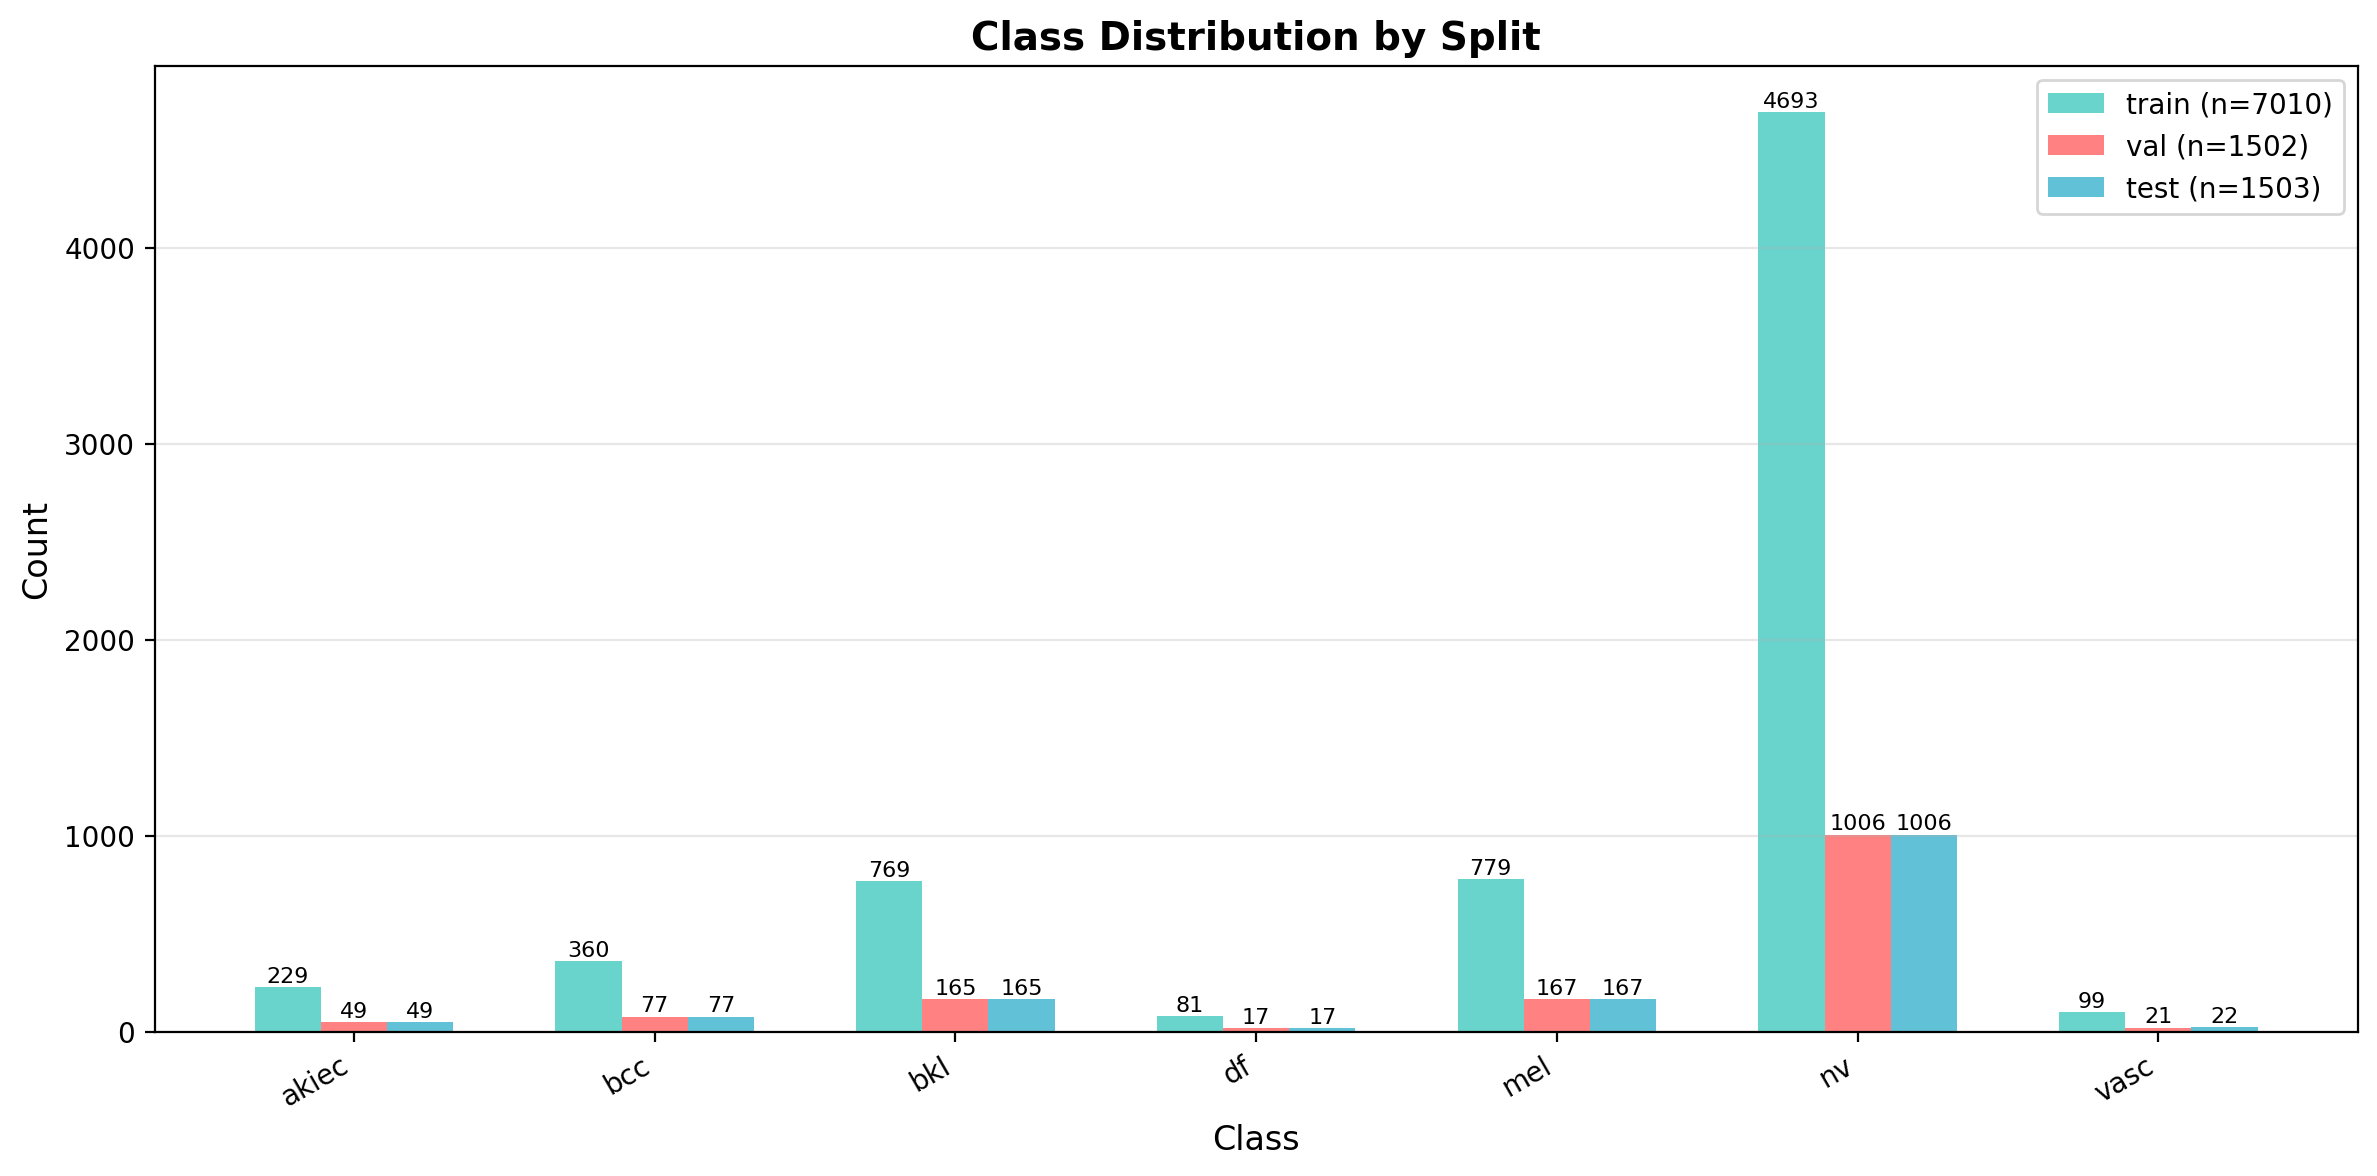
\includegraphics[width=\figwidth]{figures/class_distribution.png}
\caption{Phân bố lớp trên các tập huấn luyện, xác thực và kiểm tra. Sự mất cân bằng nghiêm trọng giữa NV và các lớp thiểu số (DF, VASC) thể hiện rõ ràng.}
\label{fig:class_distribution_vn}
\end{figure}

\section{Kiến trúc Mô hình}

Bốn kiến trúc được lựa chọn: ba CNN và một Vision Transformer. Tất cả được khởi tạo với trọng số ImageNet pretrained qua thư viện \texttt{timm} và được tinh chỉnh (fine-tune) trên ISIC 2018. Hình~\ref{fig:transfer_learning_vn} minh họa quy trình học chuyển giao này.

\begin{figure}[H]
\centering
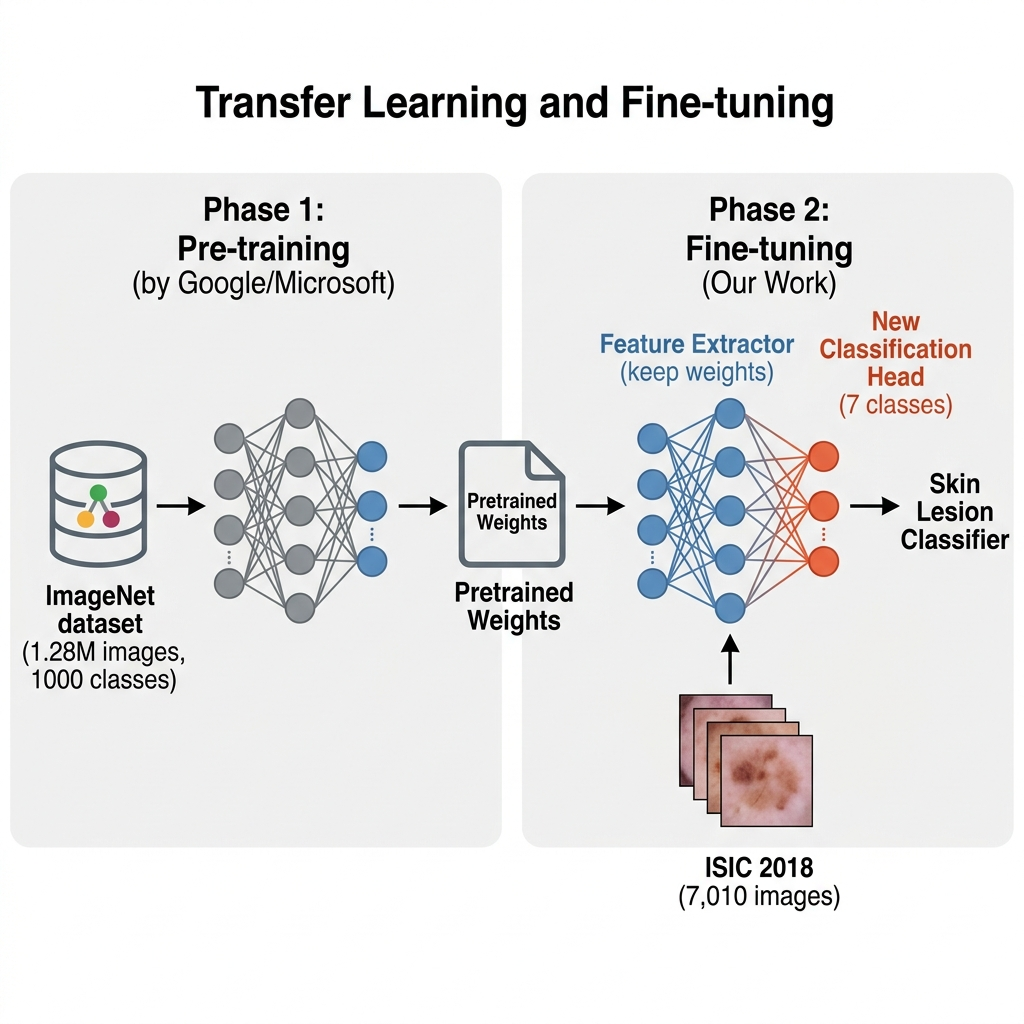
\includegraphics[width=\textwidth]{figures/transfer_learning.png}
\caption{Pipeline học chuyển giao: trọng số pretrained từ ImageNet được tải vào mỗi kiến trúc, đầu phân loại được thay thế để xuất 7 lớp tổn thương da, và toàn bộ mạng được tinh chỉnh trên tập ISIC 2018.}
\label{fig:transfer_learning_vn}
\end{figure}

\subsection{EfficientNet-B0}
Mô hình cơ sở của họ EfficientNet, thiết kế bằng Tìm kiếm Kiến trúc Thần kinh (NAS) và co giãn hỗn hợp (compound scaling). Với chỉ 5,3 triệu tham số, đạt độ chính xác cạnh tranh bằng cách tối ưu hóa đồng thời chiều sâu, chiều rộng và độ phân giải. Dropout ($p=0,3$) được thêm trước đầu phân loại.

\subsection{ResNet50}
50 lớp tổ chức thành bốn giai đoạn phần dư (residual stage). Kết nối tắt (skip connection) cho phép dòng gradient hiệu quả. 25,6 triệu tham số. Dropout ($p=0,3$).

\subsection{DenseNet121}
121 lớp với kết nối dày đặc: mỗi lớp nhận feature map được nối (concatenate) từ tất cả các lớp trước. Thúc đẩy tái sử dụng đặc trưng, giảm xuống khoảng 8 triệu tham số. Dropout ($p=0,25$).

\subsection{Swin-Tiny}
Vision Transformer phân cấp xử lý ảnh qua tự chú ý dựa trên cửa sổ dịch chuyển (shifted window). 28 triệu tham số. Tốc độ học thấp hơn ($1\times10^{-4}$), suy giảm trọng số cao hơn (0,05), warmup 5 epoch.

\begin{table}[H]
\centering
\caption{Tóm tắt bốn kiến trúc được đánh giá.}
\begin{tabular}{lrllr}
\toprule
\textbf{Mô hình} & \textbf{Tham số (M)} & \textbf{Loại} & \textbf{Đặc trưng chính} & \textbf{Dropout} \\
\midrule
EfficientNet-B0 & 5,3  & CNN & Co giãn hỗn hợp  & 0,30 \\
ResNet50        & 25,6 & CNN & Kết nối phần dư    & 0,30 \\
DenseNet121     & 8,0  & CNN & Kết nối dày đặc    & 0,25 \\
Swin-Tiny       & 28,0 & ViT & Chú ý cửa sổ dịch chuyển & 0,30 \\
\bottomrule
\end{tabular}
\end{table}

\section{Pipeline Huấn luyện}

Pipeline huấn luyện được xây dựng xung quanh một vấn đề trung tâm: mất cân bằng lớp 58:1. Bốn kỹ thuật giải quyết vấn đề này từ các góc độ khác nhau --- lấy mẫu, tăng cường dữ liệu, sửa đổi mục tiêu nhãn và điều chuẩn --- và các đóng góp cá nhân của chúng được định lượng trong nghiên cứu loại bỏ ở Chương~4. Hình~\ref{fig:training_pipeline_vn} cung cấp tổng quan toàn bộ pipeline.

\begin{figure}[H]
\centering
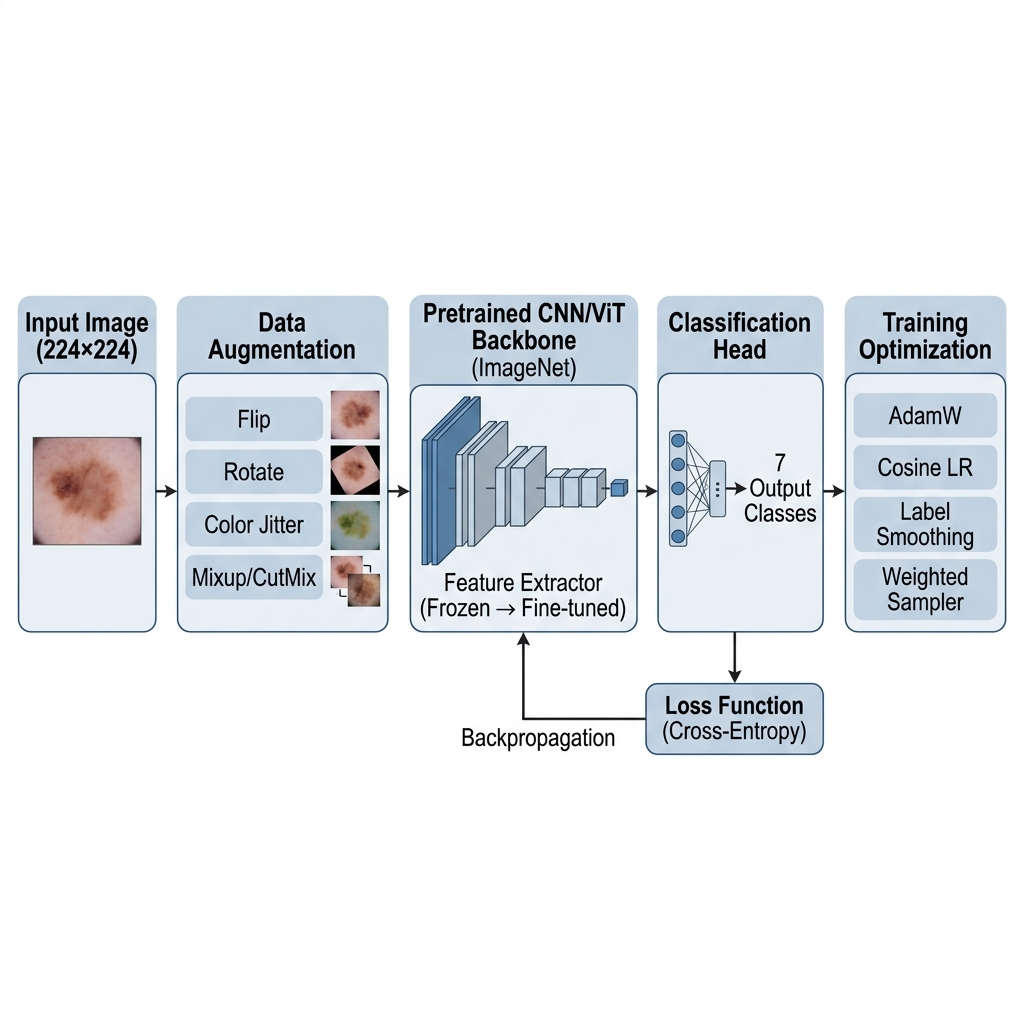
\includegraphics[width=\textwidth]{figures/training_pipeline.png}
\caption{Tổng quan pipeline huấn luyện. Ảnh đầu vào qua tăng cường dữ liệu (bao gồm Mixup/CutMix), đi qua backbone pretrained để trích xuất đặc trưng, và được phân loại bởi đầu ra. Pipeline được tối ưu với AdamW, lịch trình tốc độ học cosine, và làm mượt nhãn.}
\label{fig:training_pipeline_vn}
\end{figure}

\subsection{Lấy mẫu Ngẫu nhiên có Trọng số}

Để chống lại mất cân bằng lớp trong huấn luyện, một Weighted Random Sampler được sử dụng. Mỗi mẫu được gán một trọng số tỷ lệ nghịch với tần suất lớp của nó trong tập huấn luyện:
\begin{equation}
w_c = \frac{N}{C \cdot n_c}
\label{eq:class_weight_vn}
\end{equation}
trong đó $N$ là tổng số mẫu huấn luyện, $C$ là số lớp, và $n_c$ là số mẫu thuộc lớp $c$. Điều này đảm bảo các mini-batch xấp xỉ cân bằng lớp, ngăn mô hình phát triển thiên kiến về phía lớp đa số (NV).

\subsection{Tăng cường Mixup và CutMix}

Để điều chuẩn thêm và cải thiện tổng quát hóa, Mixup và CutMix được áp dụng với xác suất bằng nhau ($p = 0{,}5$ mỗi loại) trong huấn luyện.

\textbf{Mixup} tạo ra các ví dụ huấn luyện ảo bằng cách nội suy tuyến tính các cặp ảnh và nhãn của chúng:
\begin{equation}
\tilde{x} = \lambda x_i + (1 - \lambda) x_j, \quad \tilde{y} = \lambda y_i + (1 - \lambda) y_j
\end{equation}
với $\lambda \sim \text{Beta}(\alpha, \alpha)$ và $\alpha = 0{,}2$.

\textbf{CutMix} thay thế một vùng hình chữ nhật của một ảnh bằng vùng tương ứng từ một ảnh khác, điều chỉnh nhãn theo tỷ lệ diện tích của vùng:
\begin{equation}
\tilde{x} = M \odot x_i + (1 - M) \odot x_j, \quad \tilde{y} = \lambda y_i + (1 - \lambda) y_j
\end{equation}
trong đó $M$ là mask nhị phân chỉ vùng cắt và $\lambda$ bằng tỷ lệ vùng không bị che. CutMix alpha được đặt là 1,0.

Cả hai kỹ thuật buộc mô hình học từ các tín hiệu lai mơ hồ. Với chỉ 81 ảnh Dermatofibroma huấn luyện, huấn luyện cross-entropy thuần ghi nhớ các ví dụ đó trong vài epoch; Mixup và CutMix ngăn điều đó bằng cách đảm bảo không ví dụ huấn luyện nào có nhãn one-hot cứng.

\subsection{Làm mượt Nhãn (Label Smoothing)}

Nhãn one-hot tiêu chuẩn gán xác suất 1,0 cho lớp đúng và 0,0 cho mọi lớp khác. Label Smoothing phân phối lại một phần nhỏ khối lượng xác suất sang các lớp sai:
\begin{equation}
y_{\text{smooth}} = (1 - \epsilon) \cdot y_{\text{one-hot}} + \frac{\epsilon}{C}
\end{equation}
trong đó $\epsilon = 0{,}1$ là hệ số làm mượt và $C = 7$ là số lớp. Điều này ngăn mô hình gán xác suất 1,0 cho bất kỳ lớp nào, cải thiện calibration và, như ablation ở Chương~4 cho thấy, cải thiện Macro F1 --- mặc dù phải trả giá nhỏ về độ sắc nét AUC.

\subsection{Tối ưu hóa và Lập lịch}

Tất cả mô hình được huấn luyện với AdamW, vốn tách weight decay khỏi việc scale gradient thích nghi. Adam tiêu chuẩn hấp thụ weight decay vào các tốc độ học theo từng tham số, làm giảm hiệu lực điều chuẩn của nó; AdamW áp dụng weight decay như một hình phạt nhân tử cố định bất kể lịch sử gradient, dẫn đến tổng quát hóa tốt hơn trên dữ liệu giữ lại. Tốc độ học tuân theo lịch trình giảm cosine với khởi động tuyến tính:

\begin{itemize}
    \item \textbf{Pha khởi động} (3--5 epoch đầu): Tốc độ học tăng tuyến tính từ gần 0 lên giá trị mục tiêu. Điều này ngăn classification head được khởi tạo ngẫu nhiên tạo ra các gradient lớn làm bất ổn feature extractor pretrained trong vài cập nhật đầu.
    \item \textbf{Pha giảm cosine} (các epoch còn lại): Tốc độ học giảm theo đường cong cosine đến mức tối thiểu $1 \times 10^{-6}$, cho phép mô hình ổn định trong một vùng rộng, phẳng của loss landscape thay vì dao động quanh một minimum sắc.
\end{itemize}

\subsection{Tăng cường Dữ liệu}

Ngoài Mixup và CutMix, các phép tăng cường chuẩn sau được áp dụng trong huấn luyện:
\begin{itemize}
    \item Lật ngẫu nhiên ngang và dọc ($p = 0{,}5$)
    \item Xoay ngẫu nhiên (lên đến $\pm 90^\circ$)
    \item Color jittering (độ sáng, tương phản, độ bão hòa, hue; biên độ 0,25)
    \item Random Resized Crop (phạm vi scale: 0,85--1,0)
    \item Gaussian Blur ($p = 0{,}1$)
    \item Random Erasing ($p = 0{,}1$)
\end{itemize}

Mọi ảnh được resize về $224 \times 224$ và chuẩn hóa với mean và độ lệch chuẩn ImageNet. Batch size cố định 16 cho mọi mô hình. Giá trị này bị áp đặt bởi Swin-Tiny 28M tham số dưới huấn luyện mixed precision; giữ batch size giống nhau qua mọi kiến trúc đảm bảo bất kỳ khác biệt hiệu suất nào phản ánh chính các mô hình thay vì động lực tối ưu hóa.

\begin{table}[H]
\centering
\caption{Cấu hình siêu tham số cho từng mô hình.}
\begin{tabular}{lcccc}
\toprule
\textbf{Siêu tham số} & \textbf{EB0} & \textbf{RN50} & \textbf{DN121} & \textbf{Swin-T} \\
\midrule
Tốc độ học        & 3e-4  & 3e-4  & 2,5e-4 & 1e-4 \\
Suy giảm trọng số & 1e-3  & 1e-3  & 1e-3   & 5e-2 \\
Epoch khởi động   & 3     & 3     & 3      & 5 \\
Epoch tối đa      & 50    & 50    & 50     & 50 \\
Dừng sớm          & 12    & 12    & 12     & 12 \\
Mixup $\alpha$    & 0,2   & 0,2   & 0,2    & 0,2 \\
CutMix $\alpha$   & 1,0   & 1,0   & 1,0    & 1,0 \\
Làm mượt nhãn     & 0,1   & 0,1   & 0,1    & 0,1 \\
\bottomrule
\end{tabular}
\end{table}

\section{Các Chỉ số Đánh giá}

Accuracy một mình là chỉ số gây hiểu lầm ở đây: một bộ phân loại dự đoán Melanocytic Nevus cho mọi input đạt 67\% accuracy trong khi không phát hiện được gì có giá trị lâm sàng. Vì vậy các chỉ số sau được báo cáo song song với accuracy:

\begin{itemize}
    \item \textbf{Macro F1-Score.} Trung bình không trọng số của F1 theo lớp. Vì mỗi lớp đóng góp như nhau bất kể tần suất, một mô hình bỏ qua DF hoặc VASC bị phạt mạnh ngay cả khi accuracy tổng thể trông tốt. Đây là tiêu chí lựa chọn mô hình chính trong khóa luận này.
    \item \textbf{Weighted F1-Score.} F1 có trọng số theo cỡ lớp, đo độ chính xác tổng thể mà có tính tới mất cân bằng. Báo cáo cùng với Macro F1 cho bức tranh đầy đủ.
    \item \textbf{Macro AUC (One-vs-Rest).} Diện tích dưới đường cong ROC theo lớp, trung bình trên các lớp. AUC độc lập với ngưỡng quyết định và đo khả năng xếp hạng các trường hợp lớp dương trên các lớp âm. Trong triage lâm sàng nơi xác suất output được tiêu thụ trực tiếp để xếp hạng rủi ro, đây là chỉ số liên quan.
    \item \textbf{Cohen's Kappa ($\kappa$).} Độ đồng thuận đã hiệu chỉnh cho ngẫu nhiên. $\kappa > 0{,}6$ thường được xem là đồng thuận đáng kể.
    \item \textbf{Matthews Correlation Coefficient (MCC).} Tóm tắt toàn bộ ma trận nhầm lẫn (TP, TN, FP, FN) trong một con số duy nhất, đặc biệt phù hợp cho dữ liệu mất cân bằng vì không bị thiên kiến bởi lớp đa số.
    \item \textbf{Độ nhạy và Độ đặc hiệu theo lớp.} Độ nhạy (recall) = TP / (TP + FN); Độ đặc hiệu = TN / (TN + FP). Cả hai báo cáo theo lớp để định lượng riêng các hành vi gọi nhầm và bỏ sót.
\end{itemize}

\section{Chiến lược Kết hợp (Ensemble)}

Các phương pháp ensemble đã liên tục xuất hiện trong các bài nộp đạt kết quả cao nhất của ISIC challenge, và lý do thì đơn giản: các mô hình đa dạng phạm sai lầm ở các vị trí khác nhau, và việc lấy trung bình các output xác suất của chúng triệt tiêu một phần sai số đó. Khóa luận này sử dụng biểu quyết mềm (soft voting), lấy trung bình các vector xác suất thô trước khi lấy argmax. Hình~\ref{fig:ensemble_arch_vn} minh họa kiến trúc.

\begin{figure}[H]
\centering
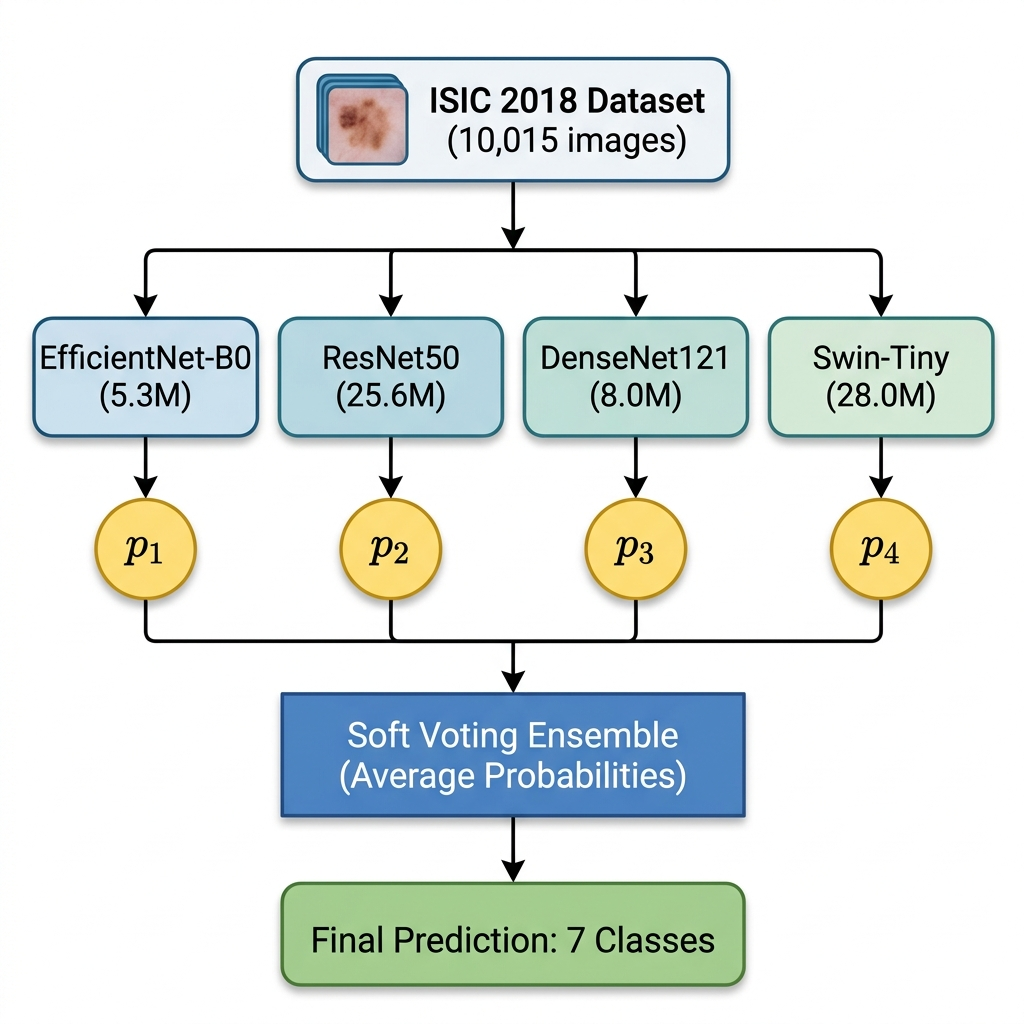
\includegraphics[width=\figwidth]{figures/ensemble_architecture.png}
\caption{Kiến trúc ensemble biểu quyết mềm. Mỗi trong bốn mô hình tạo một vector xác suất trên 7 lớp. Các vector được lấy trung bình theo từng phần tử, và lớp có xác suất trung bình cao nhất được chọn làm dự đoán cuối cùng.}
\label{fig:ensemble_arch_vn}
\end{figure}

Công thức formal:
\begin{equation}
\hat{y} = \arg\max_c \frac{1}{M} \sum_{m=1}^{M} p_m(c \mid x), \quad M = 4
\end{equation}

So với hard voting (mỗi mô hình lấy argmax rồi vote), soft voting giữ thông tin xác suất --- nó phân biệt được giữa ``cả bốn mô hình rất chắc MEL'' và ``hai mô hình vote MEL 51\%, hai mô hình vote NV 49\%''. So với stacking (meta-learner học trọng số ensemble), soft voting đơn giản hơn đáng kể, không cần val set thứ hai và không gây overfit thêm trên tập dữ liệu nhỏ.

\section{Khả năng Giải thích với Grad-CAM}

Sự chấp nhận lâm sàng của một công cụ chẩn đoán AI phụ thuộc vào nhiều hơn là độ chính xác --- một mô hình phải cung cấp lập luận có thể kiểm tra. Grad-CAM tính gradient của điểm số lớp mục tiêu $y^c$ đối với bản đồ đặc trưng tích chập cuối cùng $A^k$, và sử dụng các gradient đó để tạo bản đồ nhiệt không gian có trọng số theo kênh:
\begin{equation}
\alpha_k^c = \frac{1}{Z} \sum_i \sum_j \frac{\partial y^c}{\partial A_{ij}^k}, \quad L_{\text{Grad-CAM}}^c = \text{ReLU}\left(\sum_k \alpha_k^c A^k\right)
\end{equation}

Trong đó $\alpha_k^c$ là trọng số kênh thu được bằng global average pooling của gradient, và $L^c$ là heatmap đã ReLU (chỉ giữ phần đóng góp positive). Heatmap được up-sample về kích thước input gốc và overlay lên ảnh bằng colormap JET.

Đối với phân loại tổn thương da, Grad-CAM hoạt động như bài kiểm tra tính phản chứng: một mô hình tập trung activation vào nội thất và ranh giới tổn thương đang chú ý đến các đặc trưng mà bác sĩ nhận ra; một mô hình thắp sáng vạch ruler hoặc da nền thì không, bất kể accuracy trên test set là gì.

\chapter{Thí nghiệm và Kết quả}

Tất cả thí nghiệm được thực hiện trên một GPU NVIDIA duy nhất sử dụng huấn luyện nửa chính xác (FP16) với PyTorch 2.x. Hạt giống ngẫu nhiên cố định ở 42. Kết quả trên tập kiểm tra giữ lại.

\section{So sánh Mô hình Đơn lẻ}

\begin{table}[H]
\centering
\caption{So sánh hiệu suất trên tập kiểm tra. Giá trị tốt nhất được in \textbf{đậm}.}
\begin{tabular}{lccccc}
\toprule
\textbf{Mô hình} & \textbf{Accuracy} & \textbf{Macro F1} & \textbf{AUC} & \textbf{MCC} & \textbf{Kappa} \\
\midrule
EfficientNet-B0 & \textbf{0,8836} & \textbf{0,8311} & 0,9522 & \textbf{0,7721} & \textbf{0,7710} \\
ResNet50        & 0,8603 & 0,7902 & 0,9565 & 0,7310 & 0,7309 \\
DenseNet121     & 0,8543 & 0,7967 & 0,9587 & 0,7209 & 0,7206 \\
Swin-Tiny       & 0,8490 & 0,7855 & \textbf{0,9600} & 0,7157 & 0,7150 \\
\bottomrule
\end{tabular}
\end{table}

EfficientNet-B0 dẫn đầu mọi chỉ số phân loại cứng mặc dù có ít tham số hơn mọi mô hình khác: 5,3M so với 8M (DenseNet121), 25,6M (ResNet50) và 28M (Swin-Tiny). Macro F1 của nó đạt 0,831 vượt trội ResNet50 (0,790) tới 4,1 điểm phần trăm, dù ResNet50 có gần gấp năm lần số tham số. Điều này nhất quán với giả thuyết compound-scaling của Tan và Le: tối ưu hóa đồng thời chiều sâu, chiều rộng và độ phân giải đầu vào tạo ra một biên hiệu quả khác biệt về chất lượng thay vì các lợi ích cận biên gia tăng.\footnote{Giá trị cross-entropy loss trên test (0,75) tương đối cao cho mọi mô hình là hệ quả mong đợi của Label Smoothing: các mô hình huấn luyện với target mềm ($\epsilon=0{,}1$) xuất ra độ tin cậy tối đa khoảng $1 - \epsilon + \epsilon/C \approx 0{,}93$ thay vì 1,0, tạo giá trị loss thô cao hơn mà không phản ánh sự suy giảm chất lượng phân loại.}

Một mẫu hình nổi bật khi so sánh accuracy với AUC giữa các mô hình: chúng \textbf{đảo ngược} nhau. EfficientNet-B0 dẫn đầu về các chỉ số phân loại cứng trong khi Swin-Tiny, kém 3,5 điểm phần trăm về accuracy, tạo ra AUC cao nhất (0,960). Cơ chế tự chú ý dựa trên cửa sổ của Transformer dường như tạo ra phân phối xác suất được hiệu chỉnh tốt hơn ngay cả khi các dự đoán cứng của nó kém chính xác hơn --- có thể vì việc tích hợp ngữ cảnh toàn cục pha trộn bằng chứng khắp toàn bộ tổn thương, làm mịn các ước tính tin cậy về phía tần suất lớp thực. Lợi thế calibration này không chuyển thành quyết định rời rạc tốt hơn trên 7.010 ảnh huấn luyện, nhất quán với phát hiện rằng Vision Transformer cần dữ liệu đáng kể nhiều hơn để thu hẹp khoảng cách với CNN về phân loại cứng. Trong một ứng dụng triage lâm sàng nơi output xác suất của mô hình được tiêu thụ trực tiếp cho xếp hạng rủi ro thay vì ra quyết định nhị phân, thứ tự AUC sẽ là so sánh liên quan.

\subsection{Phân tích Theo Lớp}

Melanoma (MEL) là lớp khó nhất cho mọi kiến trúc, với F1 từ 0,625 (Swin-Tiny) đến 0,695 (EfficientNet-B0). Khó khăn này có tính cấu trúc: MEL chồng lấp với BKL về sắc tố và với NV về kết cấu, cùng sự nhập nhằng làm cho melanoma khó chẩn đoán trên lâm sàng. Các giá trị AUC kể một câu chuyện đáng khích lệ hơn --- 0,913 đến 0,930 --- chỉ ra rằng các mô hình liên tục xếp hạng các trường hợp melanoma thật trên các lựa chọn lành tính ngay cả khi ngưỡng cứng 0,5 không tách được chúng. Trong một workflow triage nơi các trường hợp được sắp xếp theo điểm rủi ro thay vì gắn cờ bằng cutoff nhị phân, thứ tự xác suất này là output có giá trị.

Dermatofibroma (DF) nằm ở thái cực ngược lại: F1 từ 0,800 đến 0,938 dù chỉ có 81 mẫu huấn luyện và 17 mẫu test. Weighted Random Sampler đảm bảo Dermatofibroma xuất hiện trong mọi mini-batch thay vì bị nhấn chìm bởi NV, và đặc trưng lâm sàng riêng biệt của DF --- một tổn thương cứng giống nút bấm với các đặc điểm dermoscopy đặc trưng --- cung cấp tín hiệu phân biệt rõ ràng. Tuy nhiên, các con số này mang phương sai cao: với 17 mẫu test, một phân loại sai bổ sung dịch chuyển F1 khoảng 0,06, nên khoảng cách rõ ràng 14 điểm giữa EfficientNet-B0 (0,938) và ResNet50 (0,800) không nên được đọc như khác biệt hiệu suất đáng tin cậy.

Vascular Lesion (VASC) được phân loại tốt một cách liên tục, với AUC đạt 1,000 cho hai kiến trúc. Sắc đỏ-tím của tổn thương mạch máu cung cấp tín hiệu màu mạnh, rõ ràng mà mọi mô hình đều nhận diện đáng tin cậy. Cũng như DF, tập test 22 mẫu nghĩa là các con số riêng lẻ có nhiễu, nhưng các giá trị AUC gần hoàn hảo ổn định qua các kiến trúc và phản ánh độ rõ ràng thị giác của lớp này.

\subsection{Động lực Huấn luyện}

\begin{figure}[H]
\centering
\begin{subfigure}{\textwidth}
    \makebox[\textwidth][c]{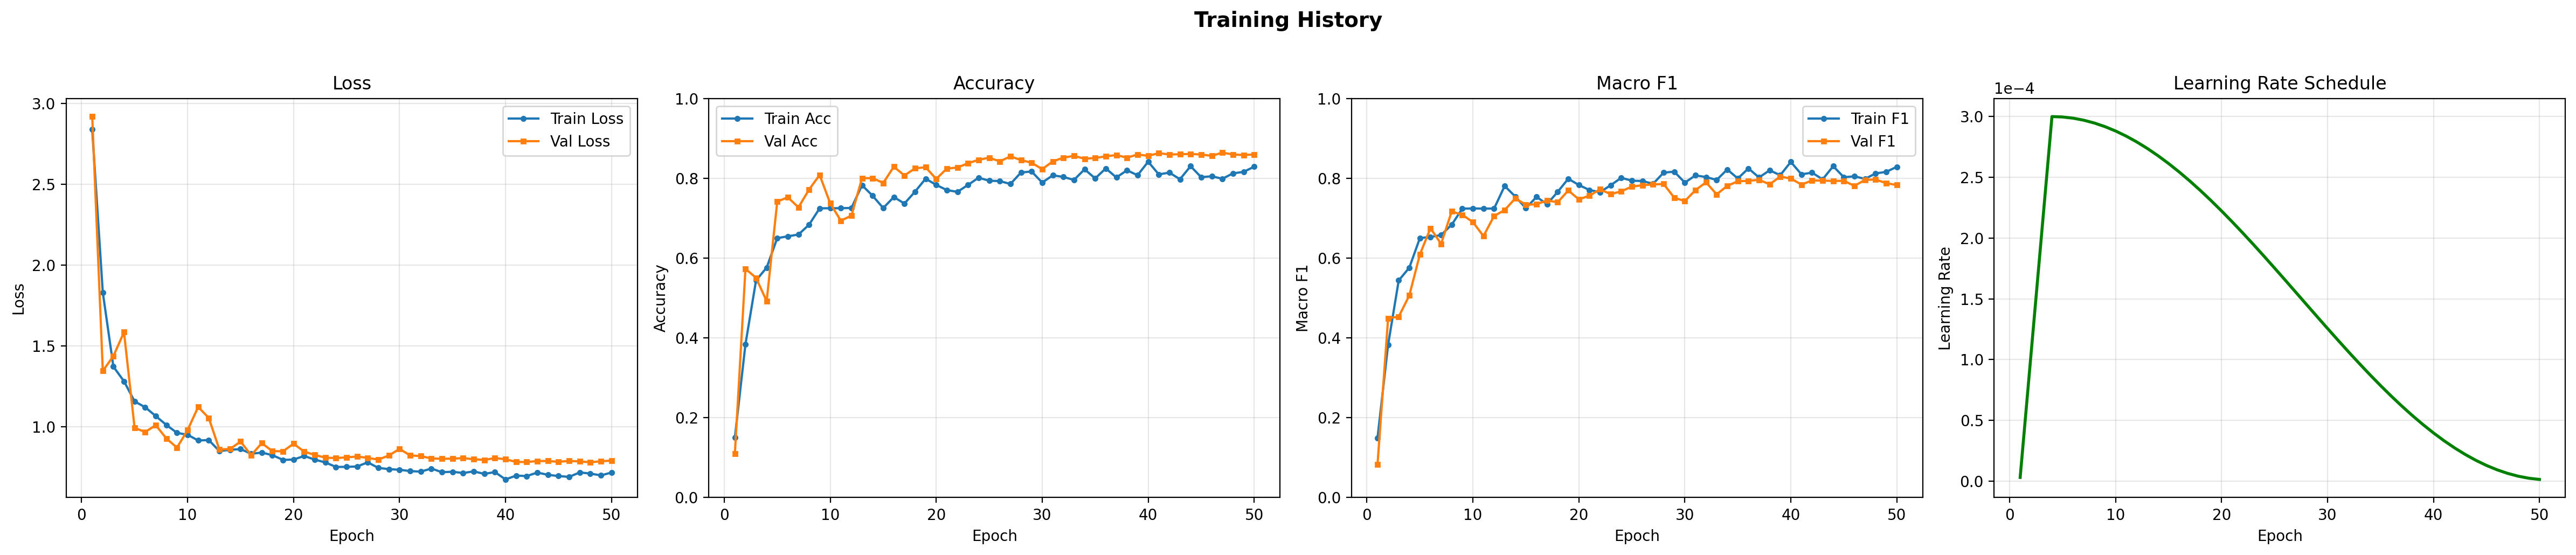
\includegraphics[width=1.15\textwidth]{figures/eb0_training_history.png}}
    \caption{EfficientNet-B0}
\end{subfigure}
\vspace{0.6cm}
\begin{subfigure}{\textwidth}
    \makebox[\textwidth][c]{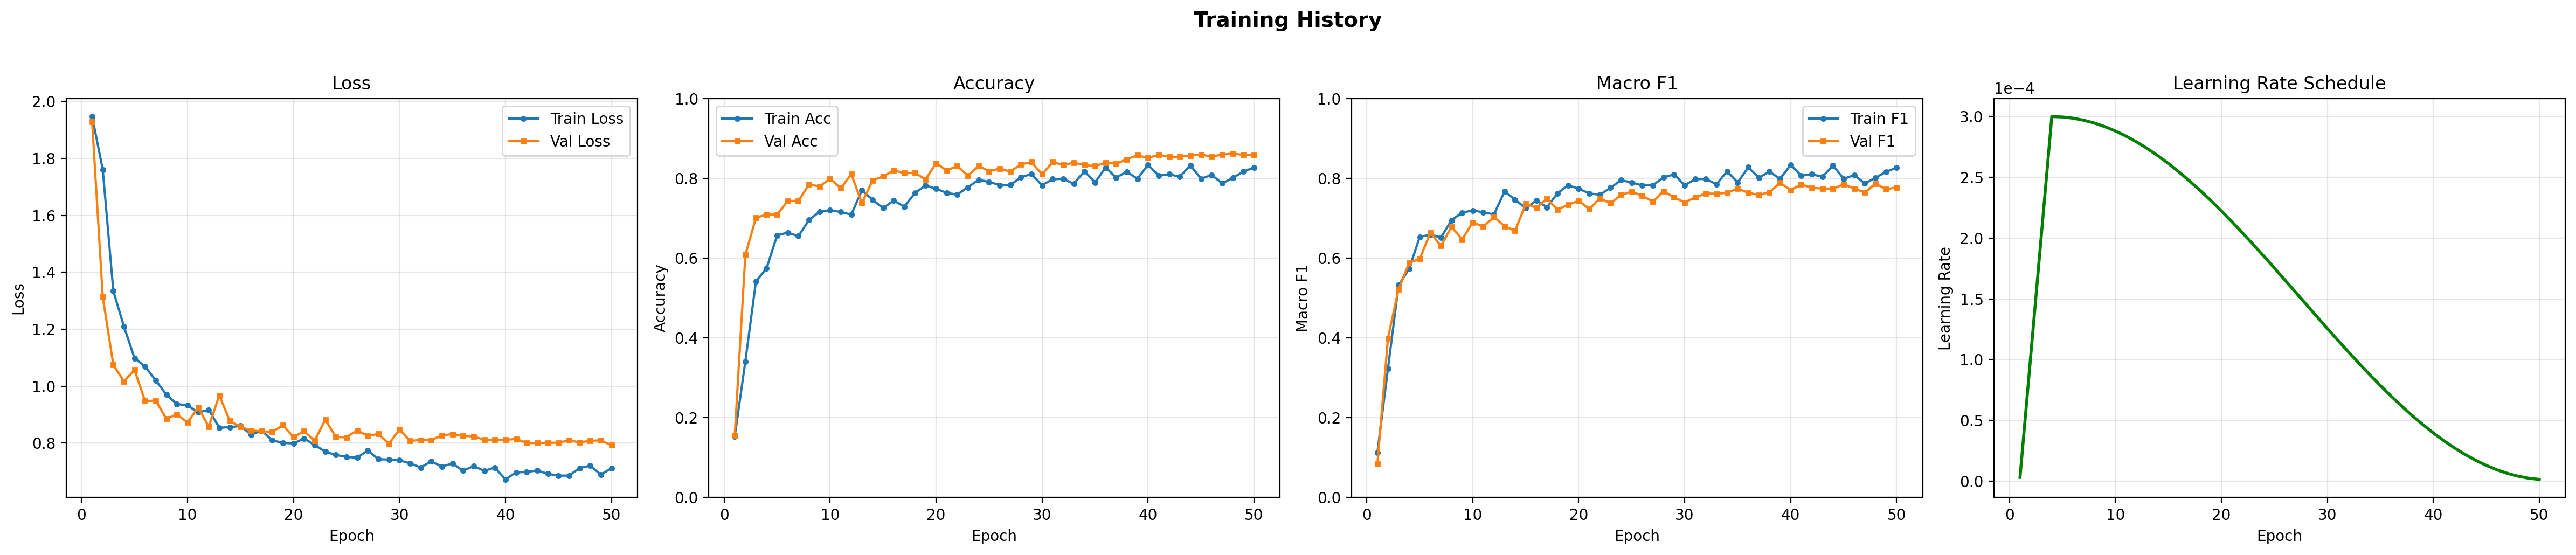
\includegraphics[width=1.15\textwidth]{figures/rn50_training_history.png}}
    \caption{ResNet50}
\end{subfigure}
\caption{Lịch sử huấn luyện: loss, accuracy và tốc độ học qua các epoch.}
\end{figure}

\begin{figure}[H]
\centering
\begin{subfigure}{\textwidth}
    \makebox[\textwidth][c]{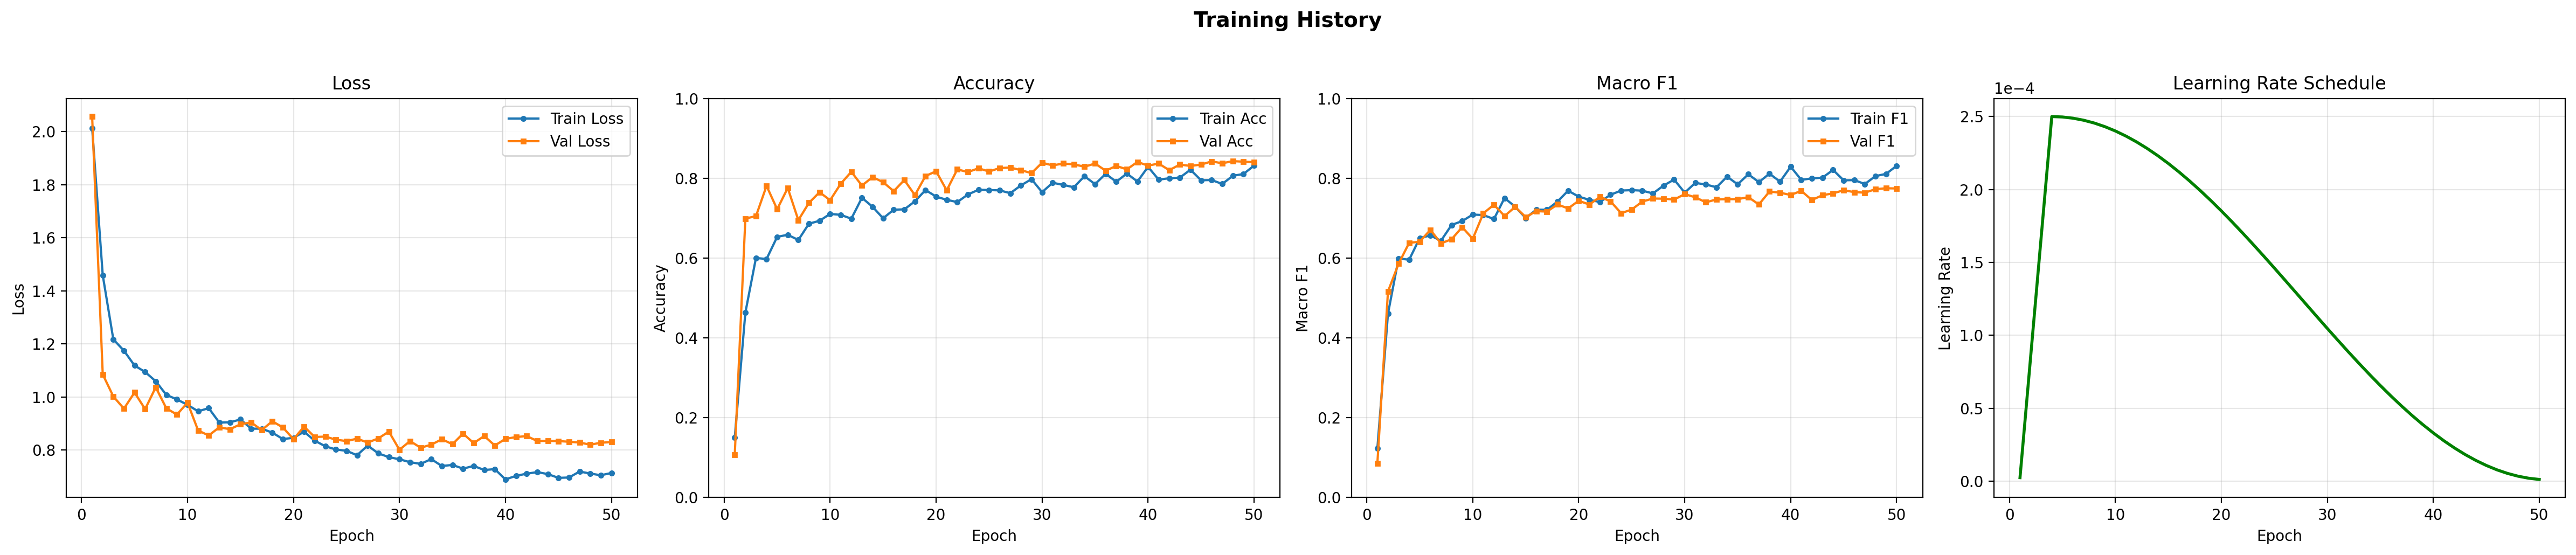
\includegraphics[width=1.15\textwidth]{figures/dn121_training_history.png}}
    \caption{DenseNet121}
\end{subfigure}
\vspace{0.6cm}
\begin{subfigure}{\textwidth}
    \makebox[\textwidth][c]{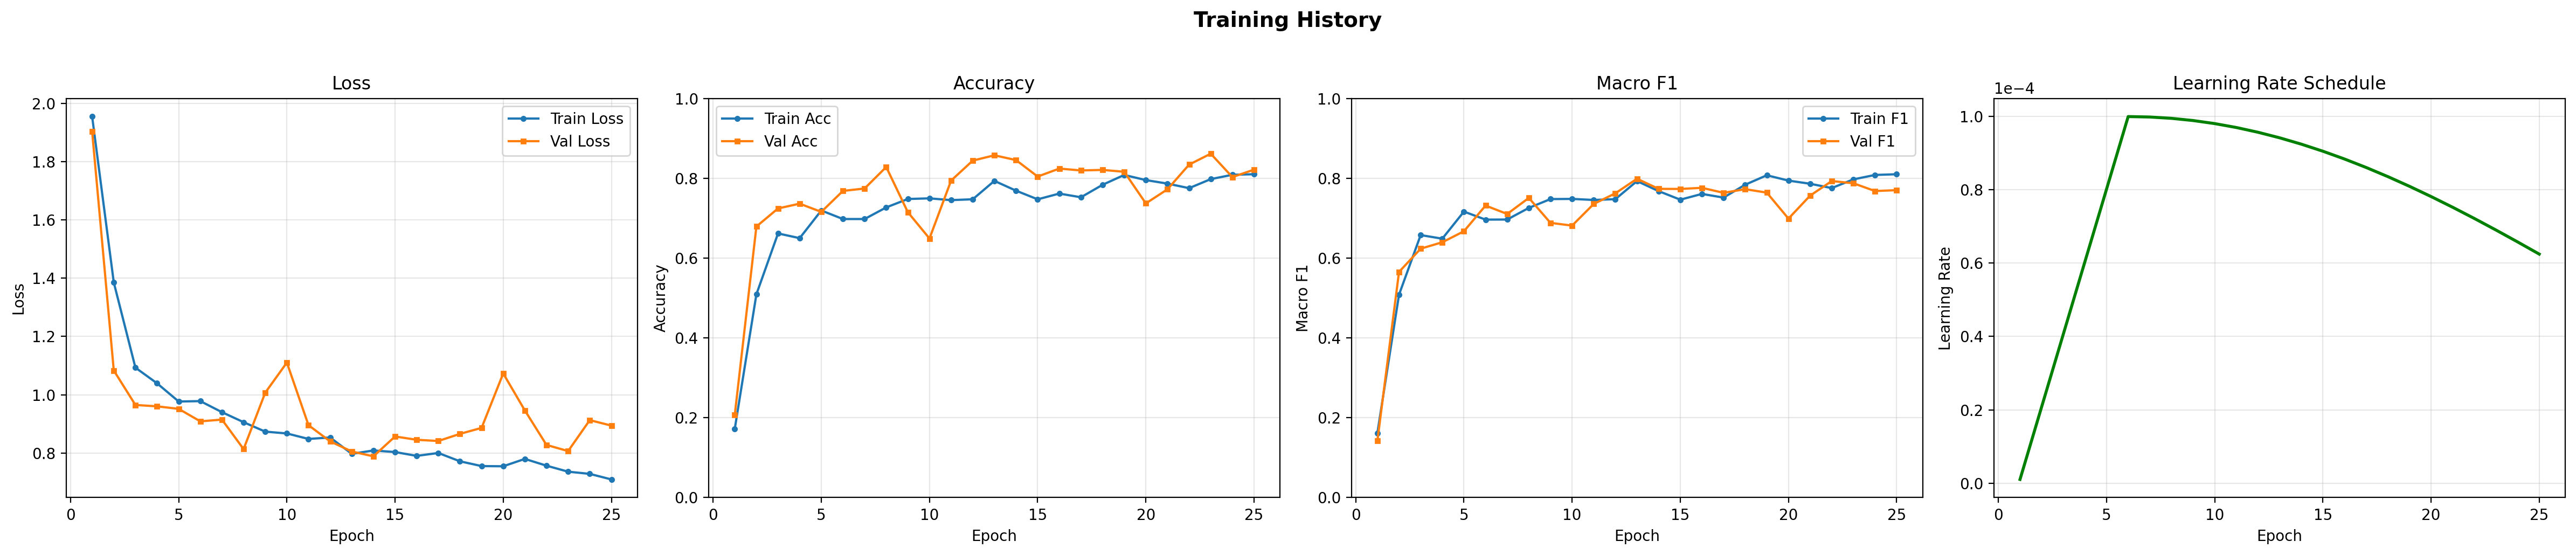
\includegraphics[width=1.15\textwidth]{figures/swin_training_history.png}}
    \caption{Swin-Tiny}
\end{subfigure}
\caption{Lịch sử huấn luyện (tiếp theo).}
\end{figure}

Tốc độ hội tụ khác nhau giữa các kiến trúc theo cách nhất quán với các tính chất đã biết của mỗi thiết kế:
\begin{itemize}
    \item EfficientNet-B0 và ResNet50 đều đạt đỉnh tại epoch 39, với dừng sớm kích hoạt sau 12 epoch tiếp theo không cải thiện.
    \item DenseNet121 đạt checkpoint tốt nhất tại epoch 49 trên 50, phản ánh xu hướng của các mạng có kết nối dày đặc cải thiện dần qua nhiều epoch khi mô hình kết nối dày đặc khai thác đầy đủ việc tái sử dụng đặc trưng.
    \item Swin-Tiny kích hoạt dừng sớm tại epoch 25 (tốt nhất tại epoch 13), tốc độ hội tụ nhanh nhất nhưng cũng là plateau sớm nhất. Điều này nhất quán với việc các mô hình Transformer dễ quá khớp hơn trên tập dữ liệu nhỏ --- warmup 5 epoch và weight decay cao hơn (0,05) làm chậm sự hội tụ ban đầu nhưng không thể bù đắp đầy đủ cho yêu cầu dữ liệu.
\end{itemize}

Tất cả các mô hình hội tụ mà không quá khớp đến mức cần can thiệp --- loss validation theo dõi loss huấn luyện xuyên suốt, xác nhận rằng tổ hợp các kỹ thuật điều chuẩn (Mixup, CutMix, Label Smoothing, Weight Decay) là đủ để ngăn sự sụp đổ về lớp đa số xuất hiện khi không có chúng.

\subsection{Ma trận Nhầm lẫn}

\begin{figure}[H]
\centering
\begin{subfigure}{\textwidth}
    \makebox[\textwidth][c]{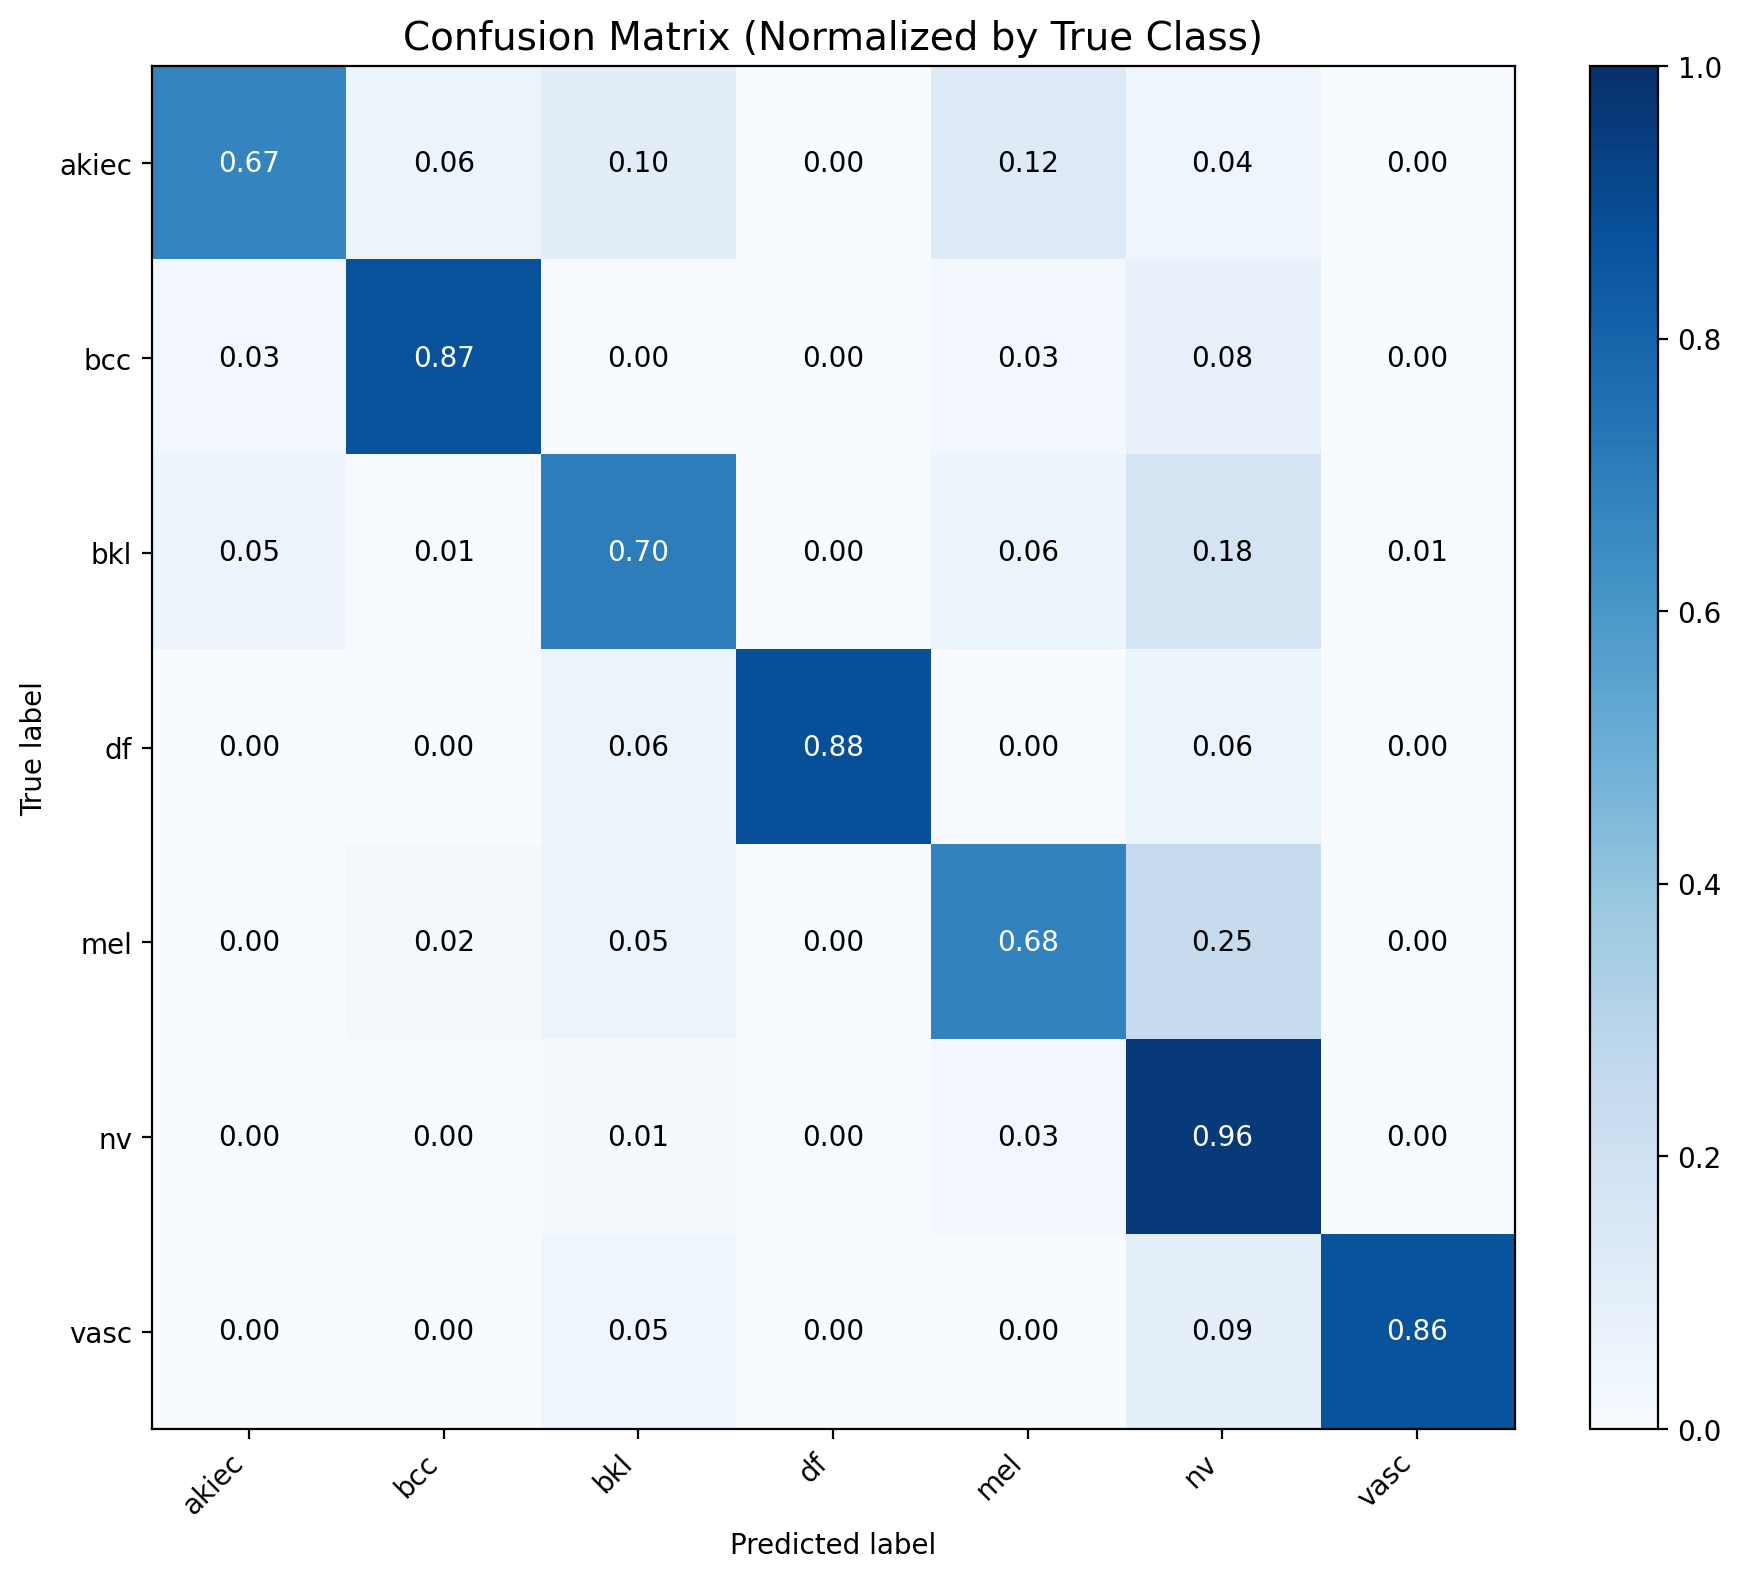
\includegraphics[width=0.9\textwidth]{figures/eb0_confusion_matrix.png}}
    \caption{EfficientNet-B0}
\end{subfigure}
\vspace{0.6cm}
\begin{subfigure}{\textwidth}
    \makebox[\textwidth][c]{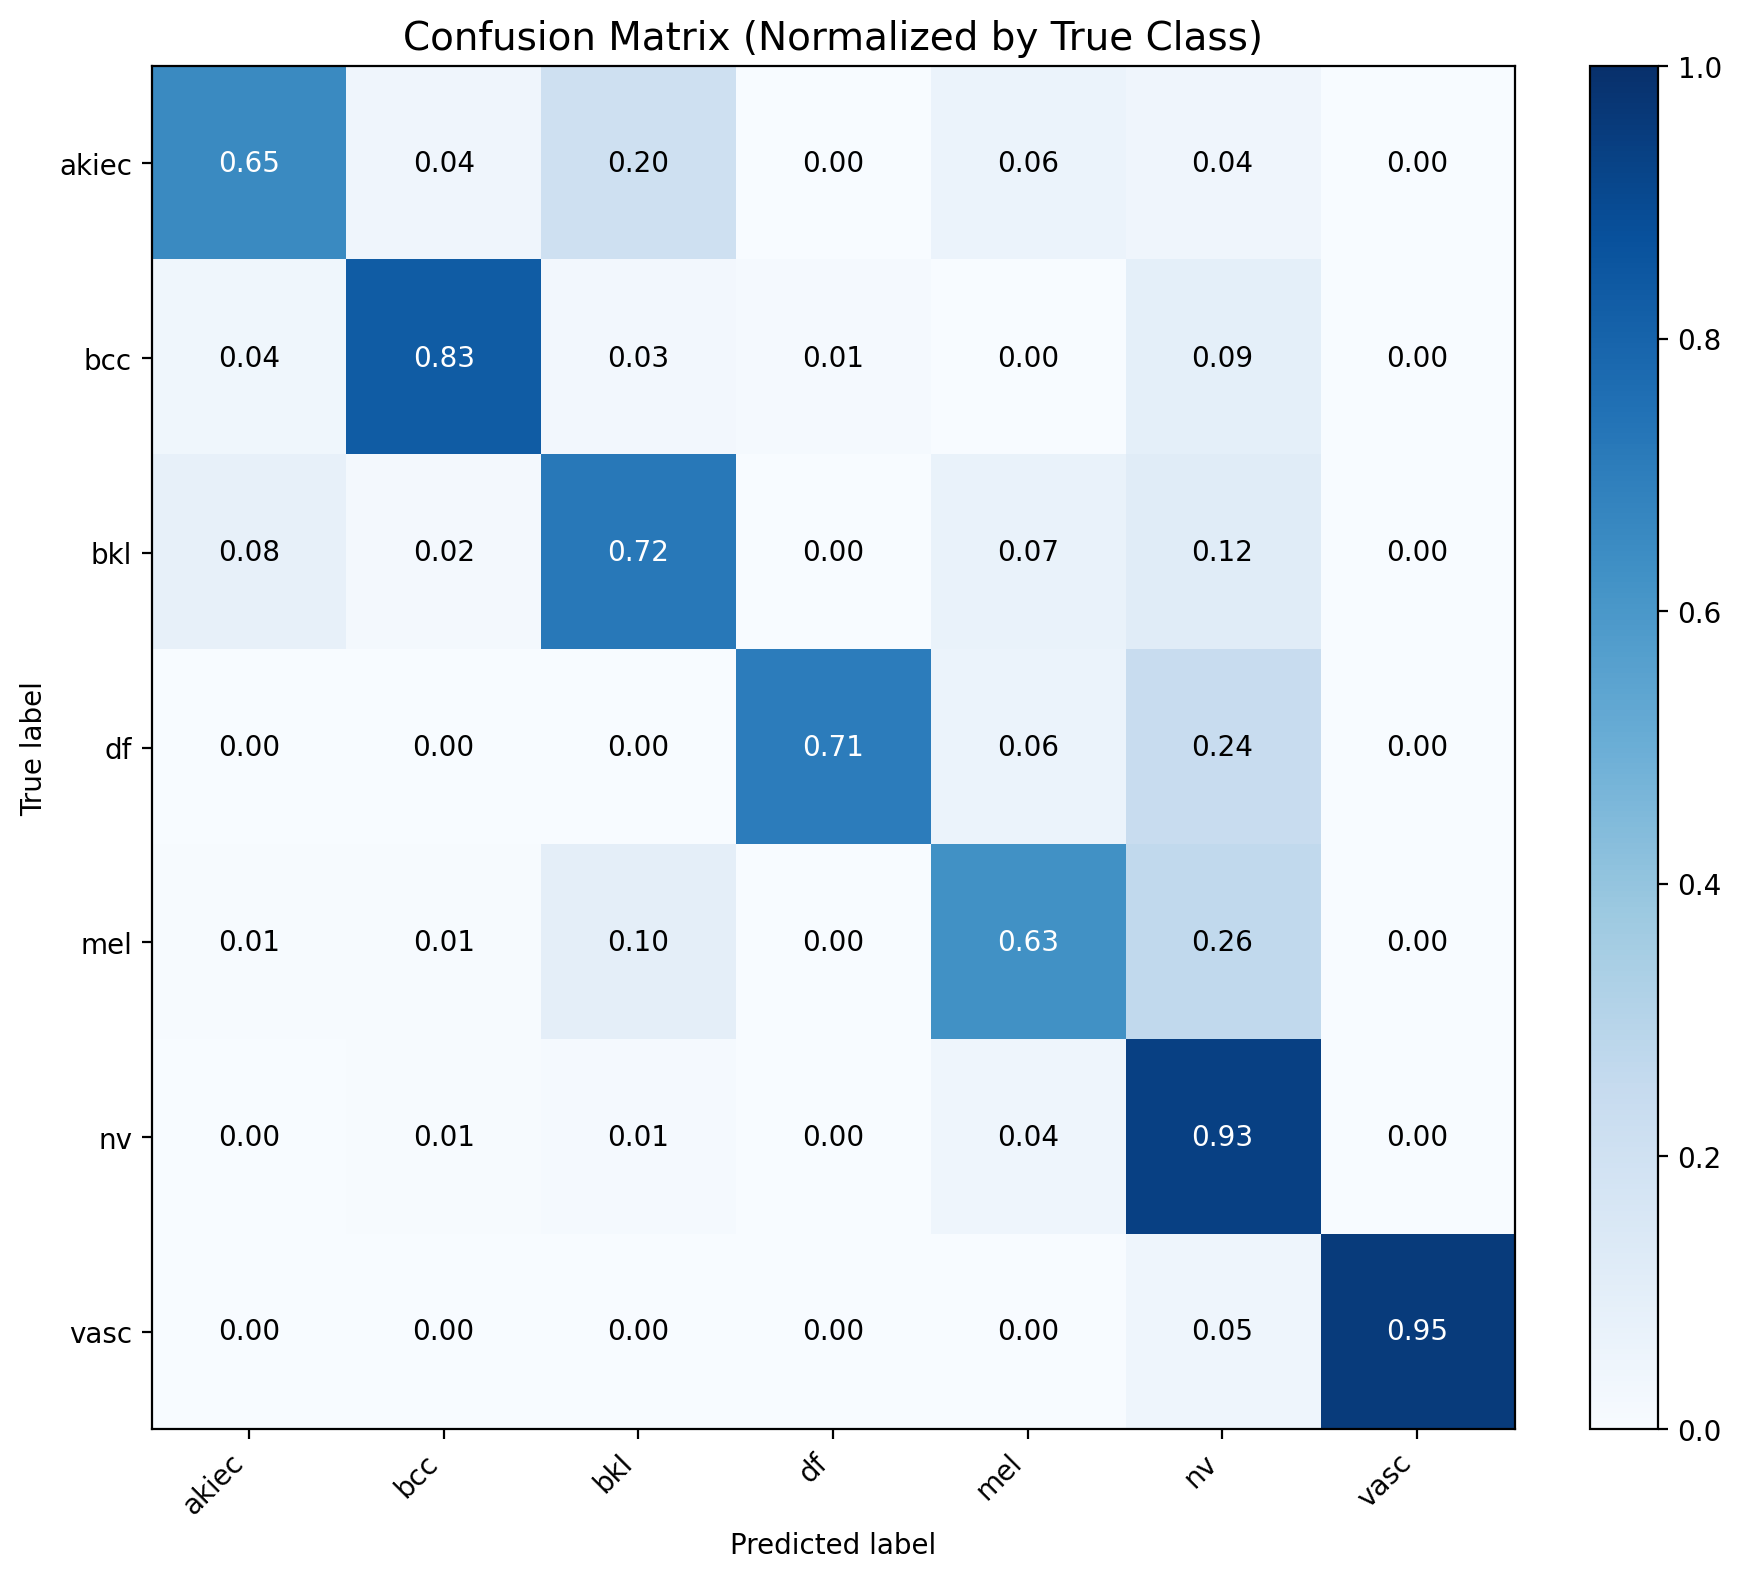
\includegraphics[width=0.9\textwidth]{figures/rn50_confusion_matrix.png}}
    \caption{ResNet50}
\end{subfigure}
\caption{Ma trận nhầm lẫn chuẩn hóa trên tập kiểm tra.}
\end{figure}

\begin{figure}[H]
\centering
\begin{subfigure}{\textwidth}
    \makebox[\textwidth][c]{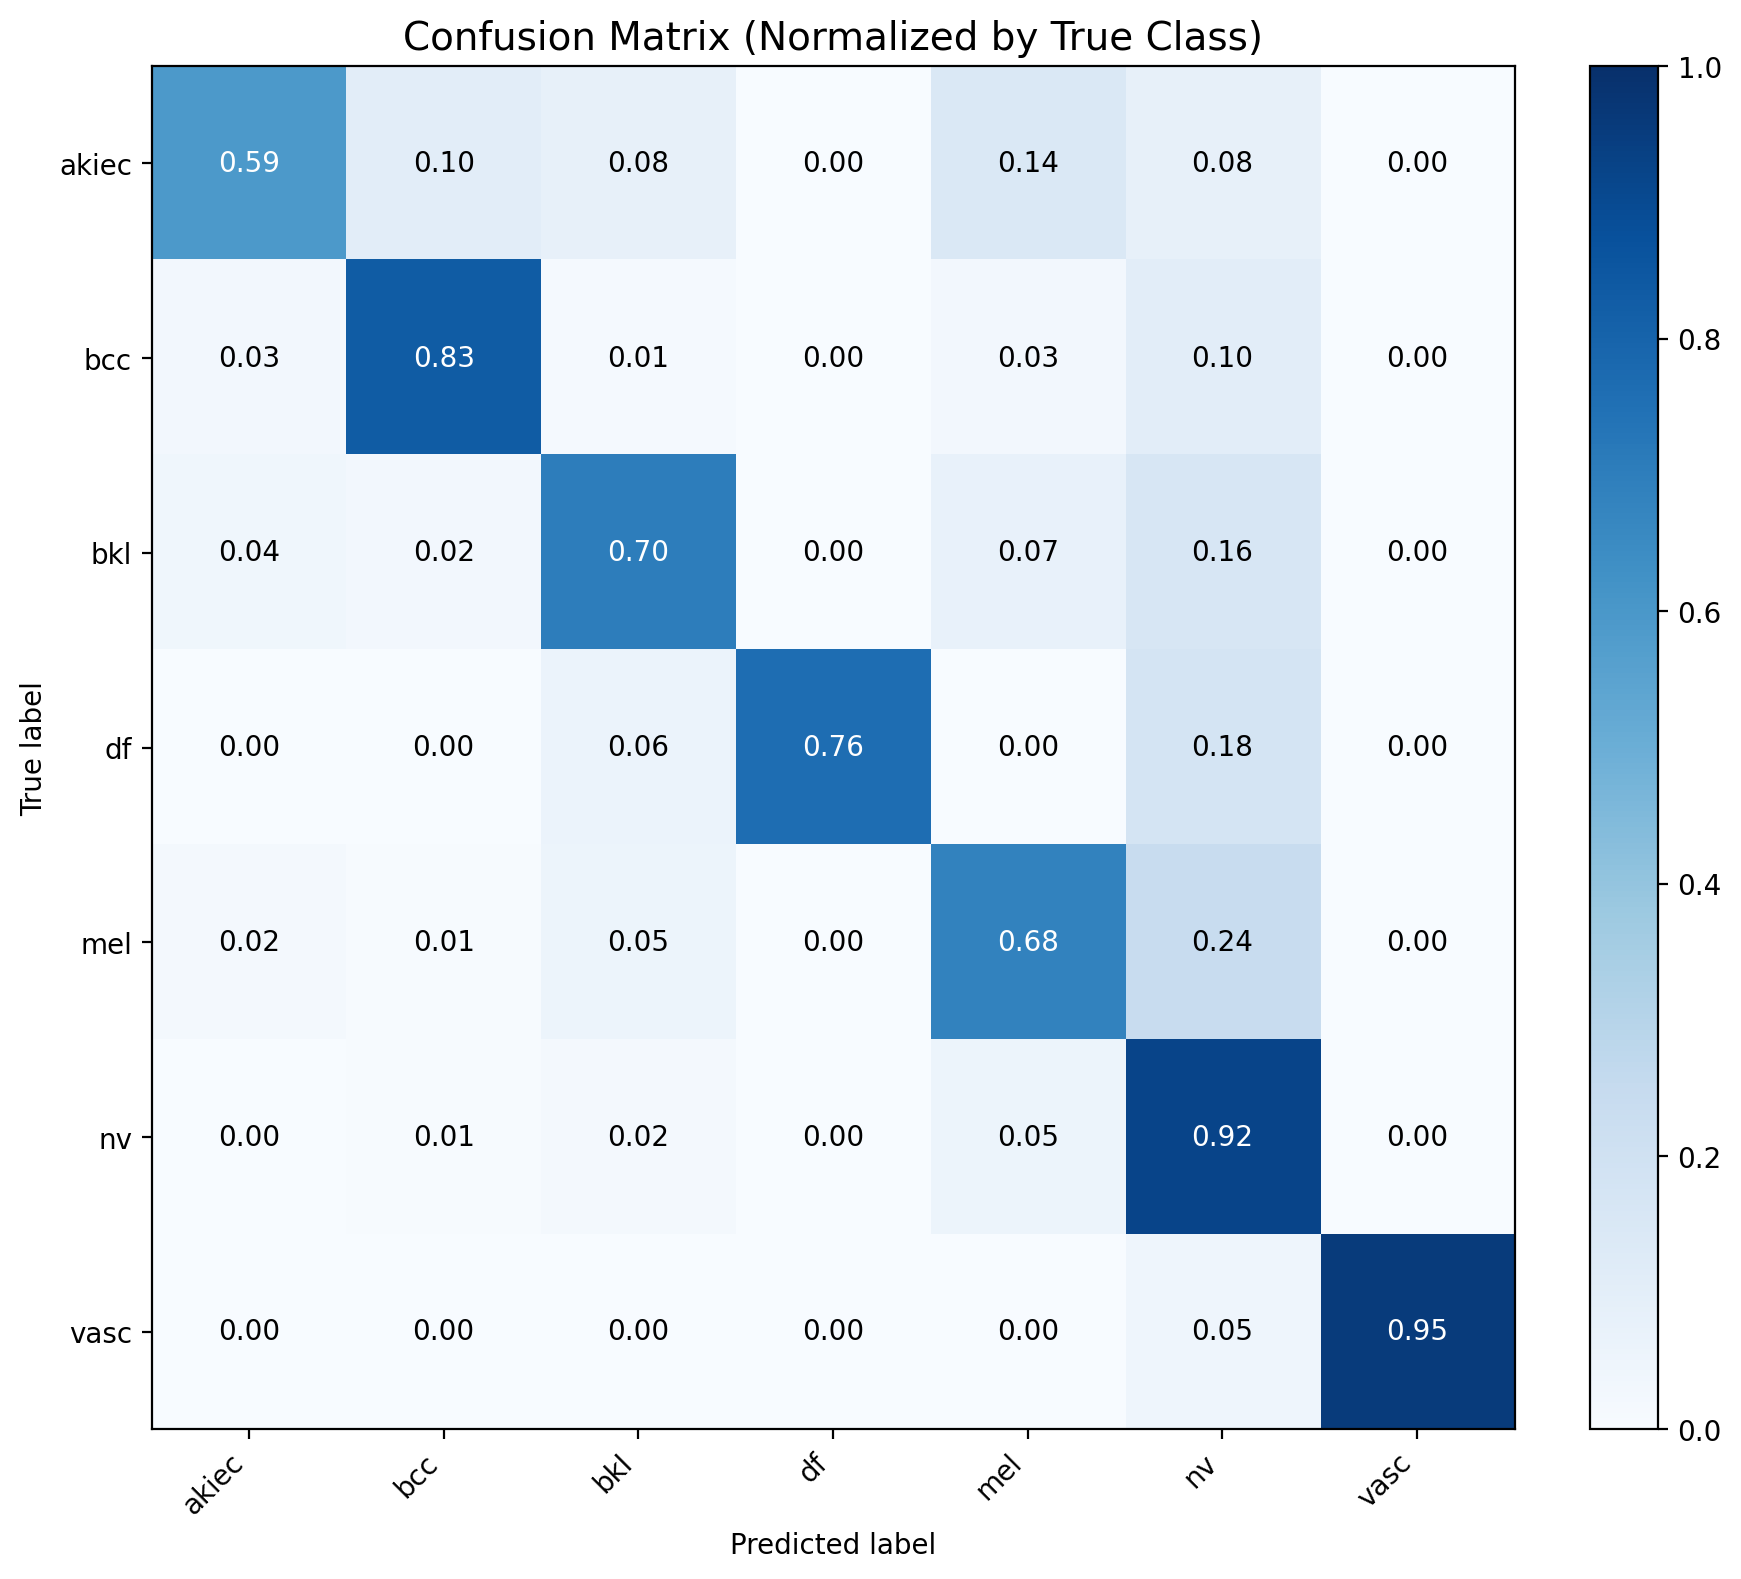
\includegraphics[width=0.9\textwidth]{figures/dn121_confusion_matrix.png}}
    \caption{DenseNet121}
\end{subfigure}
\vspace{0.6cm}
\begin{subfigure}{\textwidth}
    \makebox[\textwidth][c]{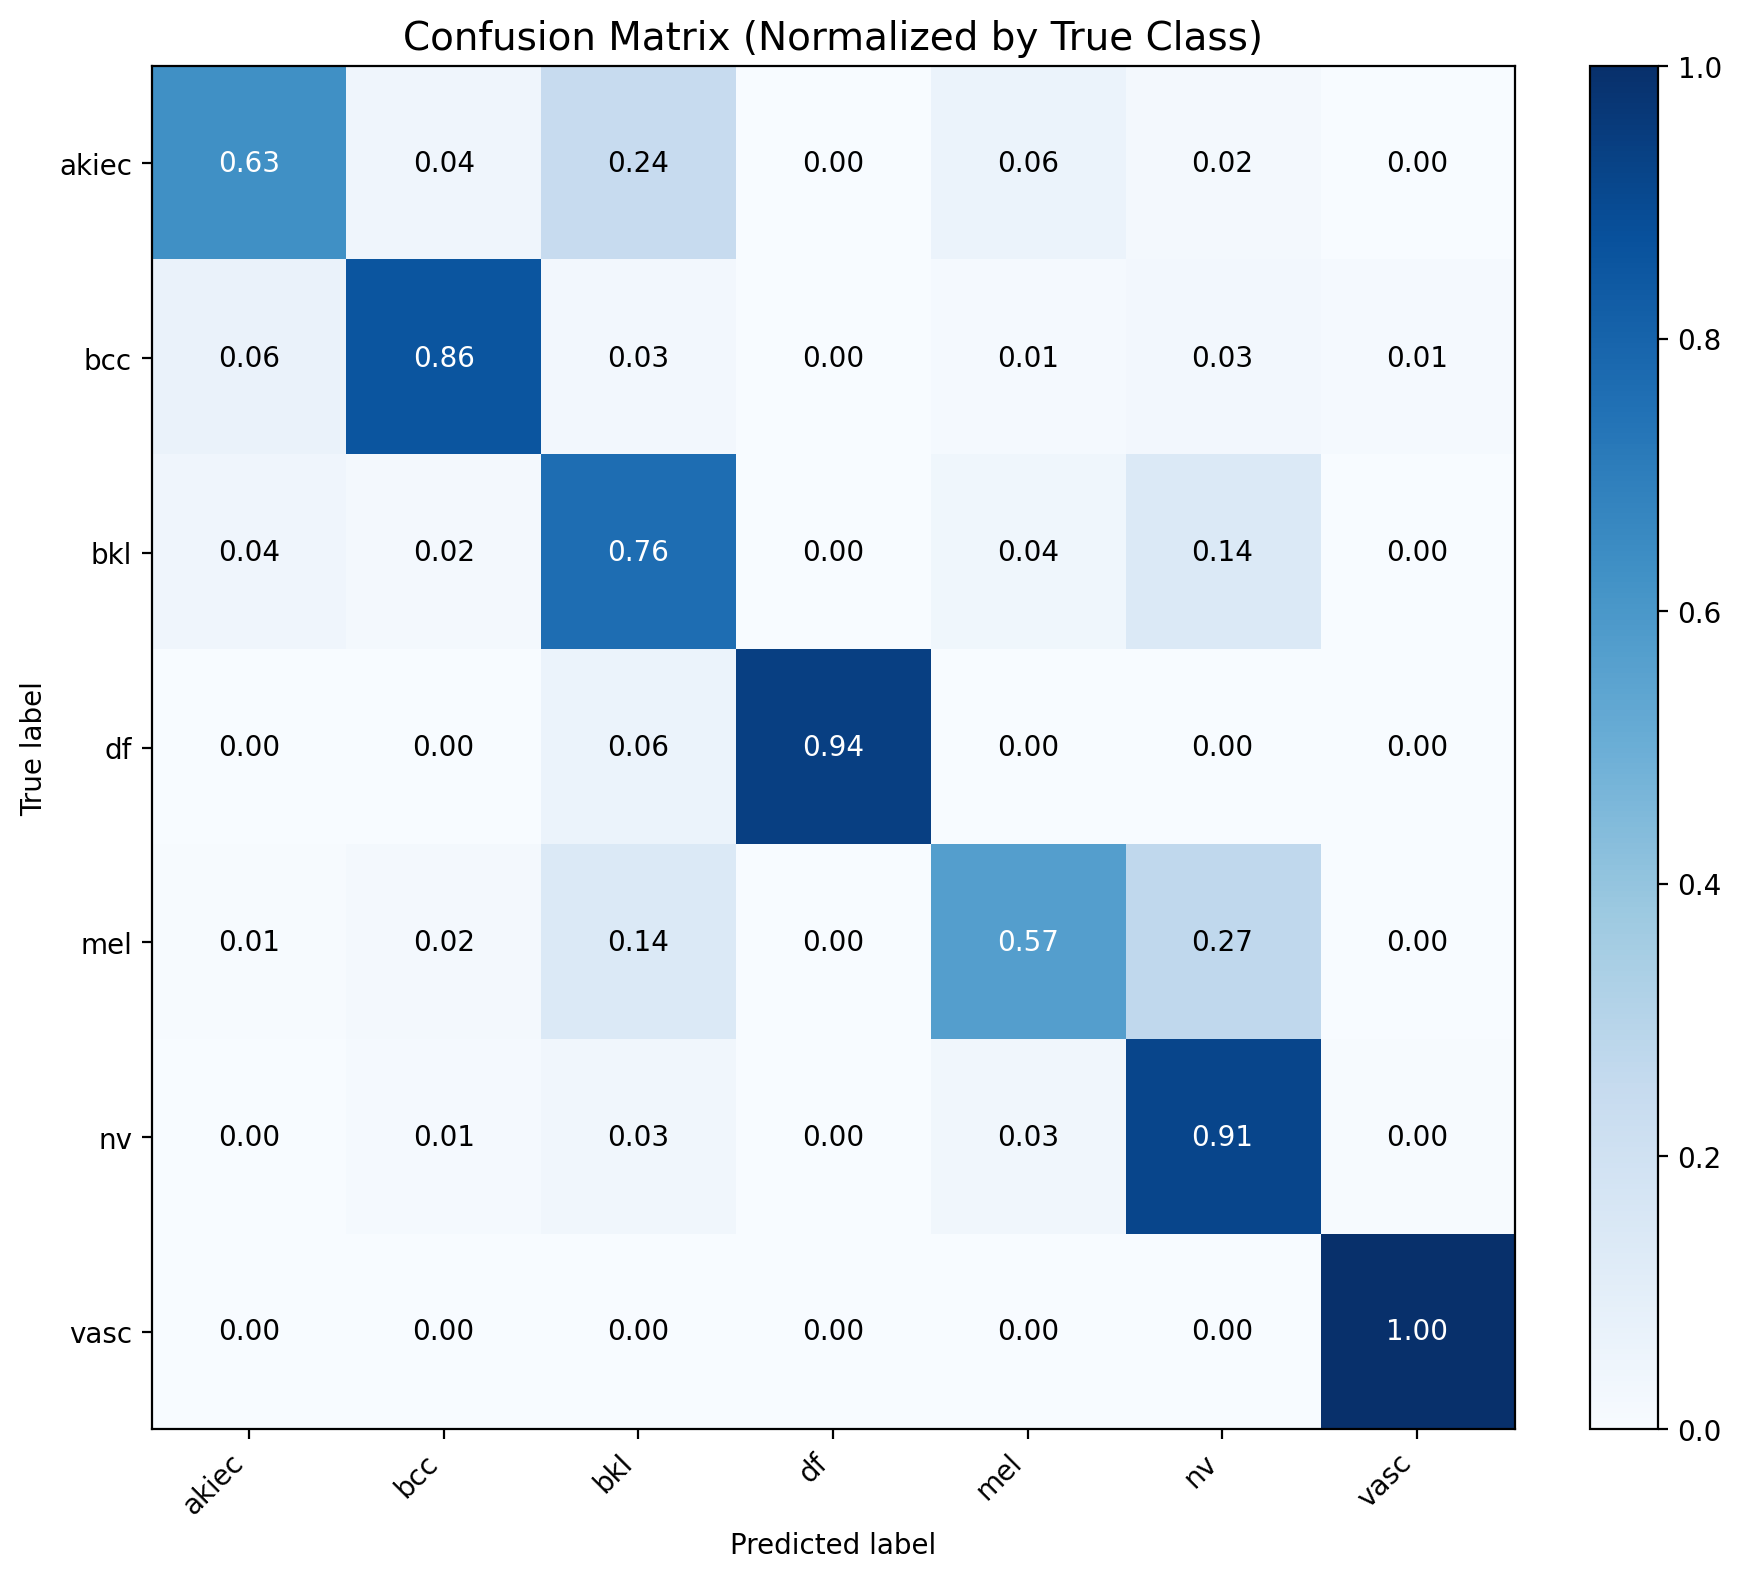
\includegraphics[width=0.9\textwidth]{figures/swin_confusion_matrix.png}}
    \caption{Swin-Tiny}
\end{subfigure}
\caption{Ma trận nhầm lẫn chuẩn hóa (tiếp theo).}
\end{figure}

Mẫu phân loại sai chiếm ưu thế trên cả bốn mô hình là MEL bị dự đoán thành NV hoặc ngược lại --- một phản ánh trực tiếp của sự chồng lấp hình thái giữa melanoma giai đoạn sớm và nốt ruồi lành tính. BKL là mục tiêu nhầm lẫn phổ biến thứ hai cho MEL. Các mẫu hình này xuất hiện nhất quán bất kể kiến trúc và khớp với xếp hạng độ khó lâm sàng đã biết trong da liễu. Quan trọng là, không mô hình nào thể hiện chế độ thất bại sụp đổ về NV cho input không phải NV: Weighted Random Sampler đảm bảo các mẫu lớp thiểu số được thấy đủ thường xuyên trong huấn luyện để ranh giới quyết định cho mỗi lớp được học có ý nghĩa.

\section{Kết quả Ensemble}

\begin{table}[H]
\centering
\caption{So sánh mô hình đơn lẻ và ensemble trên tập kiểm tra.}
\begin{tabular}{lccccc}
\toprule
\textbf{Mô hình} & \textbf{Accuracy} & \textbf{Macro F1} & \textbf{AUC} & \textbf{MCC} & \textbf{Kappa} \\
\midrule
EfficientNet-B0  & 0,8836 & 0,8311 & 0,9522 & 0,7721 & 0,7710 \\
ResNet50         & 0,8603 & 0,7902 & 0,9565 & 0,7310 & 0,7309 \\
DenseNet121      & 0,8543 & 0,7967 & 0,9587 & 0,7209 & 0,7206 \\
Swin-Tiny        & 0,8490 & 0,7855 & 0,9600 & 0,7157 & 0,7150 \\
\midrule
\textbf{Ensemble (4 mô hình)} & \textbf{0,8949} & \textbf{0,8446} & \textbf{0,9802} & \textbf{0,7956} & \textbf{0,7949} \\
\bottomrule
\end{tabular}
\end{table}

Ensemble nâng accuracy thêm 1,1 điểm phần trăm so với EfficientNet-B0 và, một cách thực chất hơn, đẩy Macro AUC từ 0,952 lên 0,980. Lợi ích AUC là kết quả có ý nghĩa hơn: nó nghĩa là xếp hạng xác suất của ensemble đáng tin cậy đúng ngay cả cho các trường hợp MEL/NV mơ hồ nơi quyết định cứng ở ngưỡng cố định thất bại. F1 melanoma cải thiện từ 0,695 (EfficientNet-B0 đơn lẻ) lên 0,744, một lợi ích 4,9 điểm có ý nghĩa lâm sàng đáng kể vì hậu quả của việc bỏ sót melanoma.

\begin{figure}[H]
\centering
\begin{subfigure}{0.46\textwidth}
    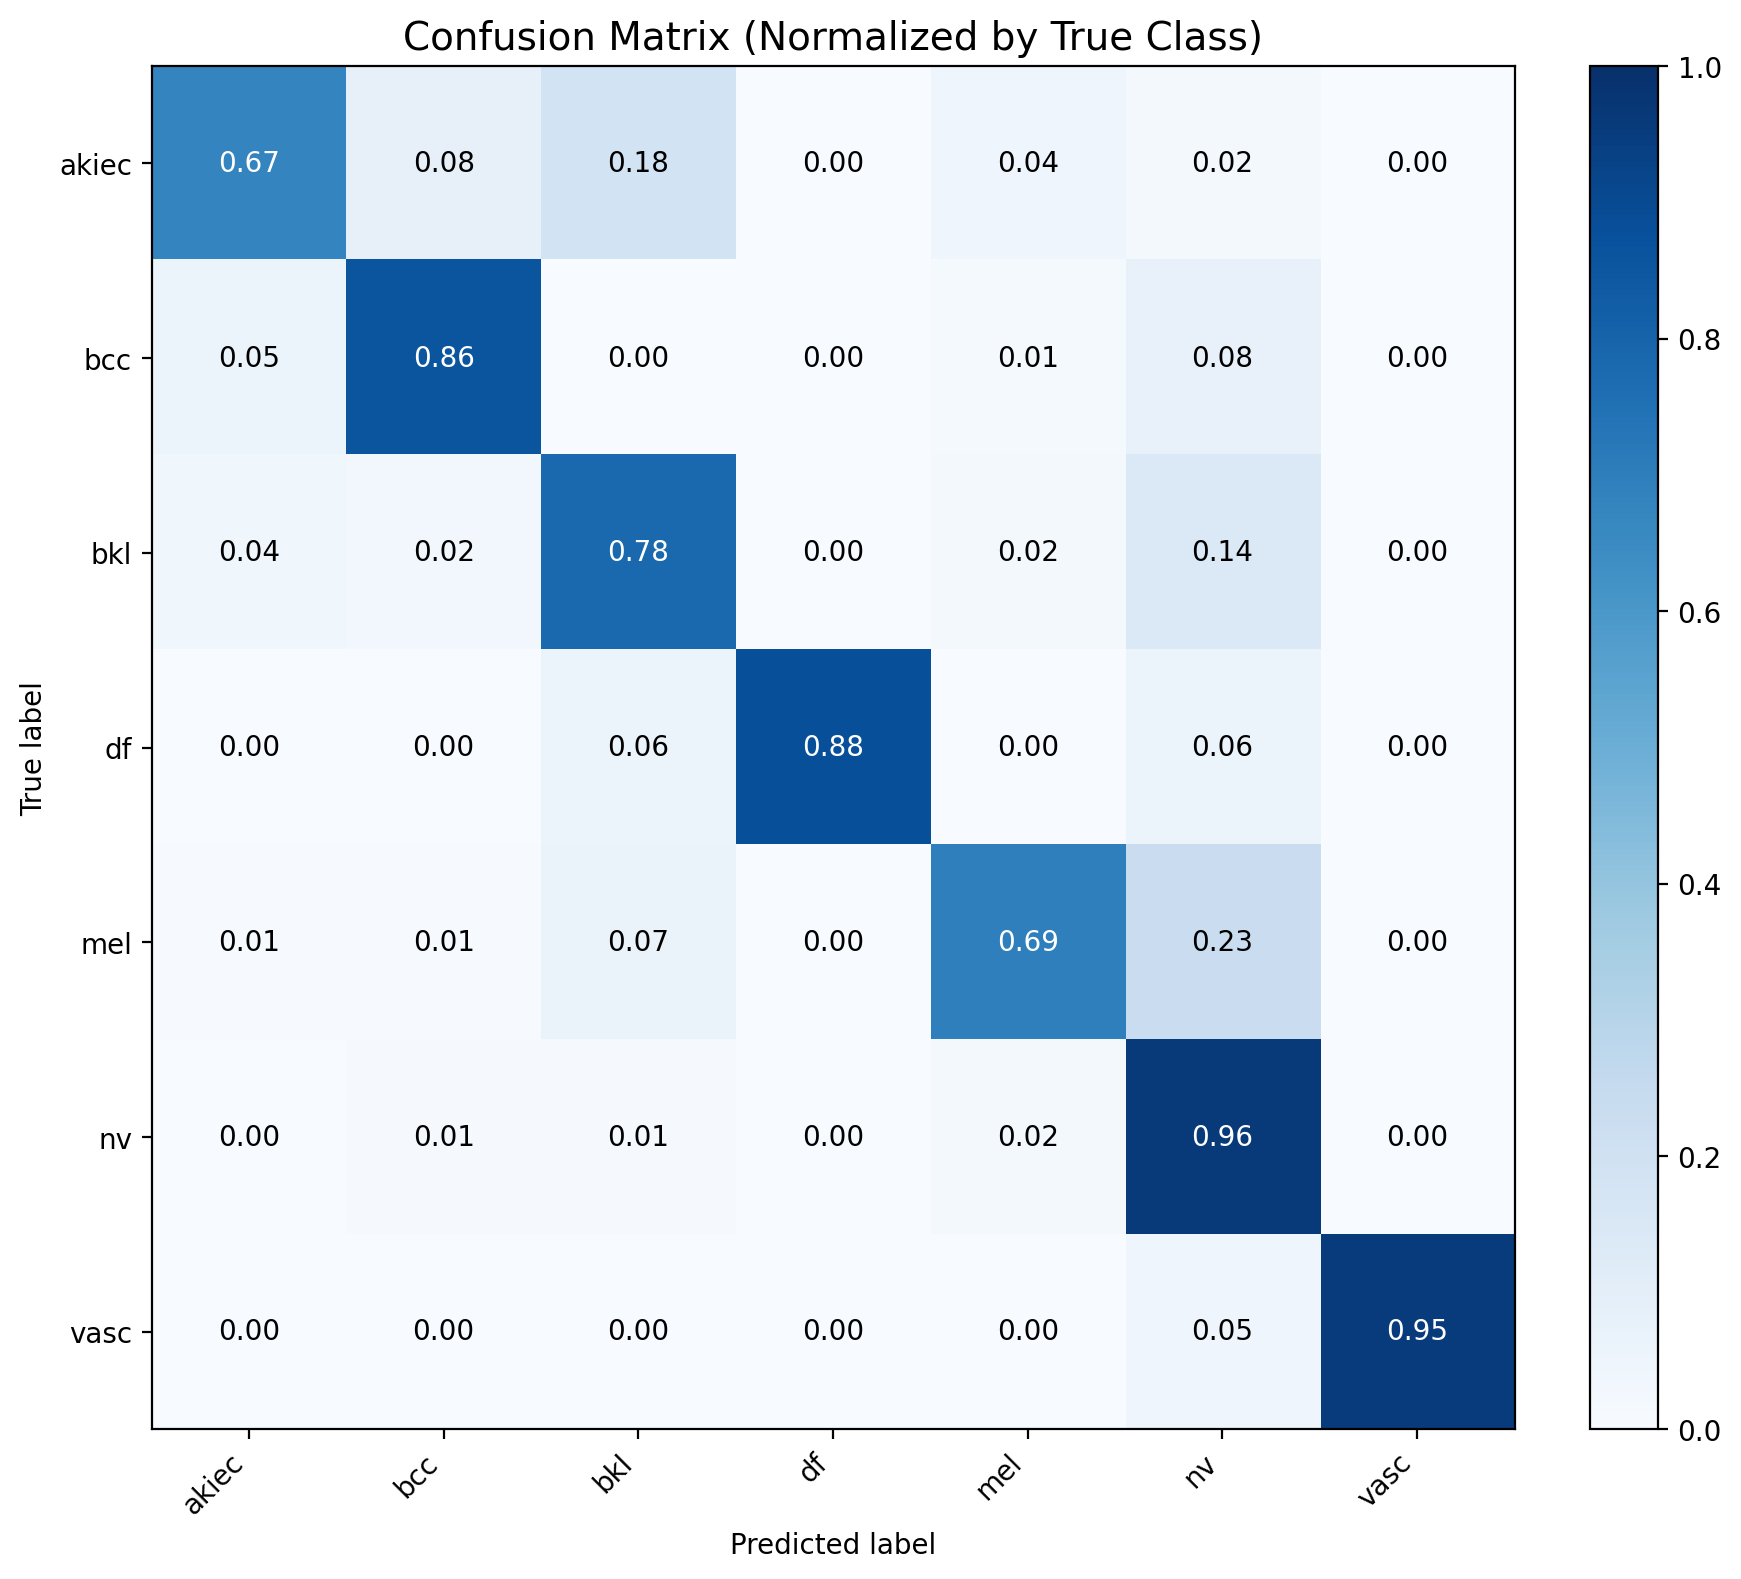
\includegraphics[width=\textwidth]{figures/ensemble_confusion_matrix.png}
    \caption{Ma trận nhầm lẫn}
\end{subfigure}
\hfill
\begin{subfigure}{0.46\textwidth}
    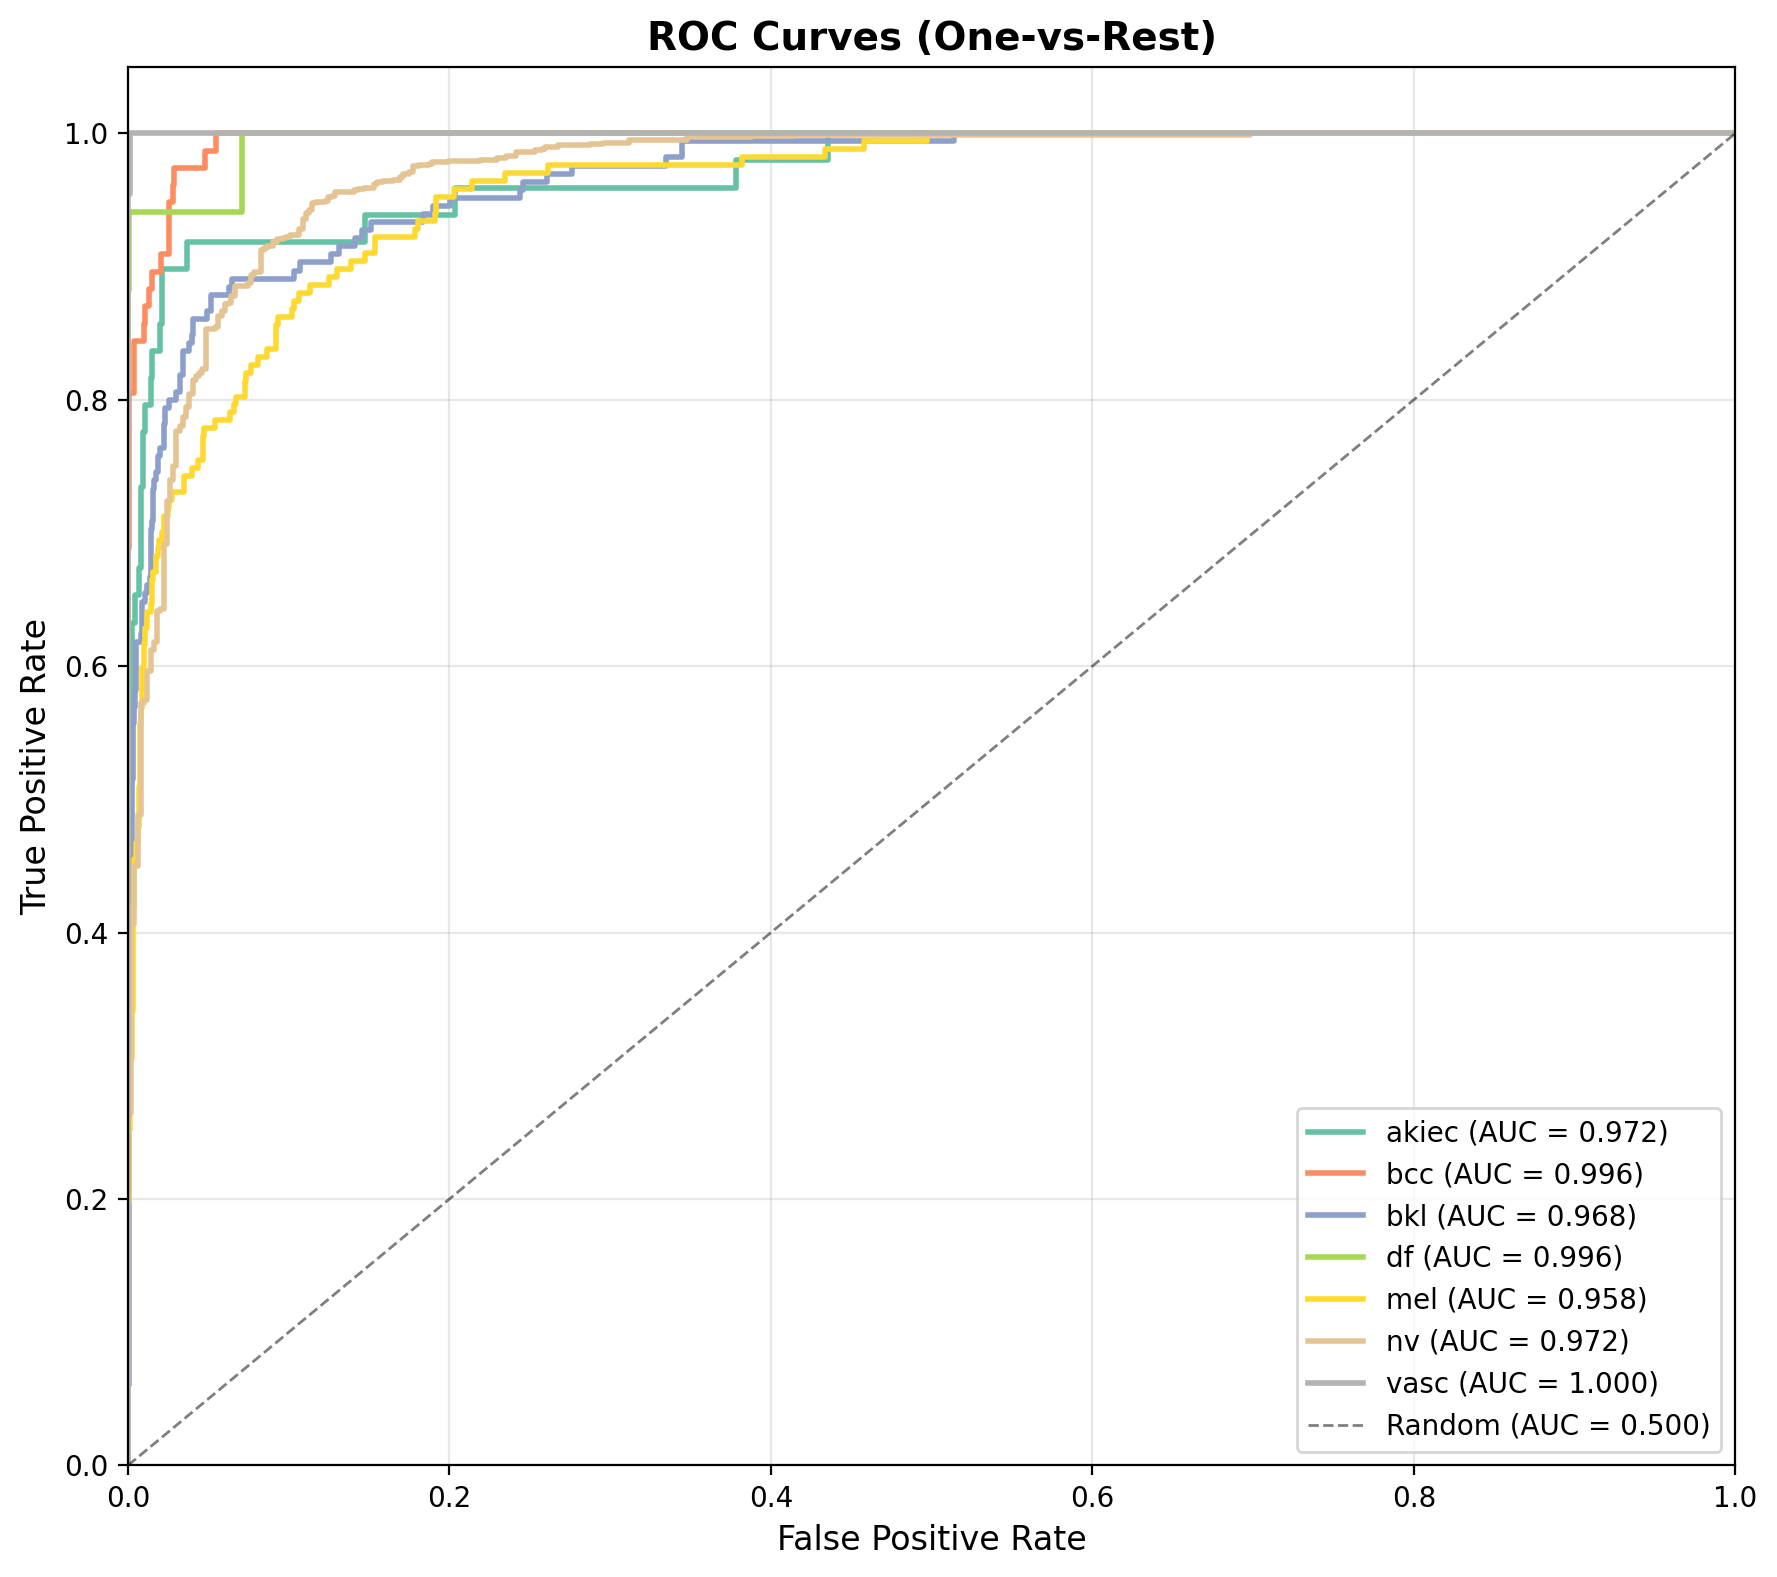
\includegraphics[width=\textwidth]{figures/ensemble_roc_curves.png}
    \caption{Đường cong ROC}
\end{subfigure}
\caption{Hiệu suất mô hình ensemble: (a) ma trận nhầm lẫn chuẩn hóa và (b) đường cong ROC theo lớp.}
\end{figure}

Ensemble cải thiện AUC cho \textbf{mọi lớp} không có ngoại lệ. F1 phân loại cứng pha trộn hơn: BCC và AKIEC giảm nhẹ (lần lượt 0,040 và 0,007) trong khi BKL, MEL, NV và VASC đều cải thiện. Các giảm F1 phản ánh một trade-off ensemble đã biết --- trung bình xác suất làm mềm các dự đoán cá nhân tự tin nhất, có thể dịch chuyển các trường hợp ranh giới theo hai hướng. Sự cải thiện AUC đơn điệu vì việc trung bình các phân phối bảo toàn thứ tự xếp hạng đồng thời giảm phương sai trong sai số mô hình cá nhân.

\section{Độ tin cậy thống kê qua các hạt giống ngẫu nhiên}

Để kiểm chứng kết quả ensemble không phải may mắn của một hạt giống khởi tạo, toàn bộ pipeline được lặp lại với năm hạt giống độc lập (\{42, 1337, 2024, 7, 11\}). CuDNN dùng kernel không tất định và Mixup/CutMix lấy mẫu ngẫu nhiên nên mỗi hạt giống nhiễu hoàn toàn quỹ đạo tối ưu hóa. Bảng~\ref{tab:multiseed_vn} báo cáo trung bình $\pm$ độ lệch chuẩn qua năm lần chạy.

\begin{table}[H]
\centering
\caption{Hiệu năng đa hạt giống ($n=5$ hạt giống). Độ lệch chuẩn của ensemble nhỏ hơn rõ rệt so với bất kỳ mô hình đơn nào --- biểu quyết mềm hấp thụ phương sai cấp hạt giống.}
\label{tab:multiseed_vn}
\begin{tabular}{lccc}
\toprule
\textbf{Mô hình} & \textbf{Accuracy} & \textbf{Macro F1} & \textbf{Macro AUC} \\
\midrule
EfficientNet-B0  & $87{,}31 \pm 1{,}32\%$ & $0{,}814 \pm 0{,}022$ & $0{,}965 \pm 0{,}006$ \\
ResNet50         & $86{,}31 \pm 0{,}57\%$ & $0{,}792 \pm 0{,}011$ & $0{,}949 \pm 0{,}003$ \\
DenseNet121      & $85{,}62 \pm 2{,}42\%$ & $0{,}797 \pm 0{,}025$ & $0{,}960 \pm 0{,}004$ \\
Swin-Tiny        & $88{,}33 \pm 1{,}96\%$ & $0{,}839 \pm 0{,}030$ & $0{,}966 \pm 0{,}008$ \\
\midrule
\textbf{Ensemble} & $\mathbf{89{,}93 \pm 0{,}66\%}$ & $\mathbf{0{,}852 \pm 0{,}010}$ & $\mathbf{0{,}982 \pm 0{,}001}$ \\
\bottomrule
\end{tabular}
\end{table}

Hai nhận xét chính. Thứ nhất, kết quả 89,49\% accuracy đã báo cáo ở phần trước nằm trong một độ lệch chuẩn của trung bình đa hạt giống 89,93\%, xác nhận đây là hiệu năng điển hình chứ không phải may mắn. Độ lệch chuẩn accuracy của ensemble (0,66 điểm phần trăm) nhỏ hơn tất cả mô hình đơn (0,57--2,42 điểm), độ lệch AUC chỉ $\pm 0{,}001$ --- gần như không đáng kể.

Thứ hai, trung bình accuracy của Swin-Tiny (88,33\%) khi qua nhiều hạt giống hé lộ rằng đây mới thực sự là mô hình đơn mạnh nhất, không phải EfficientNet-B0 như xếp hạng hạt giống 42 gợi ý. Lần chạy Swin với hạt giống 42 đã early-stop tại một điểm validation không thuận lợi (đó là kết quả 84,90\%). Khi trung bình hóa qua các hạt giống, attention toàn cục của Swin thực sự cạnh tranh với các CNN; điểm yếu là phương sai, không phải hiệu năng trung bình. Đây cũng là lý do giữ Swin trong ensemble: chính phương sai cao --- yếu tố hại cho điểm số đơn --- lại làm cho lỗi của nó ít tương quan với lỗi của các CNN, biến nó thành thành phần ensemble có giá trị.

Để kiểm định ưu thế của ensemble so với mô hình đơn mạnh nhất có ý nghĩa thống kê hay không, kiểm định McNemar được áp dụng trên bảng cặp bất đồng giữa dự đoán của (mô hình đơn, ensemble) cho mỗi hạt giống, kết quả tổ hợp qua phương pháp Fisher.

\begin{table}[H]
\centering
\caption{Kiểm định McNemar trên dự đoán tập kiểm tra, mô hình đơn so với ensemble. Cột ``Ensemble thắng'' đếm số hạt giống ensemble có nhiều mẫu đúng (đối với cặp bất đồng) hơn mô hình đơn.}
\label{tab:mcnemar_vn}
\begin{tabular}{lccc}
\toprule
\textbf{Mô hình đơn vs.\ Ensemble} & \textbf{Ensemble thắng} & \textbf{Có ý nghĩa $\alpha=0{,}05$} & \textbf{$p$ Fisher tổ hợp} \\
\midrule
EfficientNet-B0 & 5/5 & 4/5 & $5{,}3 \times 10^{-18}$ \\
ResNet50        & 5/5 & 5/5 & $4{,}5 \times 10^{-31}$ \\
DenseNet121     & 5/5 & 5/5 & $6{,}7 \times 10^{-39}$ \\
Swin-Tiny (mạnh nhất) & 5/5 & 3/5 & $1{,}2 \times 10^{-7}$ \\
\bottomrule
\end{tabular}
\end{table}

Ensemble vượt mọi mô hình đơn trên cả năm hạt giống. So với các CNN, chênh lệch rất lớn: hàng chục ảnh test ensemble đúng và mô hình đơn sai, đối lại chỉ vài ảnh ngược lại --- tổ hợp p-value dưới $10^{-18}$. So với Swin-Tiny --- mô hình đơn mạnh nhất --- mức độ chênh lệch nhỏ hơn nhưng kết luận giống nhau: ưu thế của ensemble tồn tại qua hiệu chỉnh đa kiểm định và không phải hiệu ứng ngẫu nhiên.

\section{Kết hợp metadata bệnh nhân}

Pipeline chỉ-ảnh bỏ qua ba thuộc tính mà bác sĩ da liễu nào cũng cân nhắc trước khi đưa ra chẩn đoán: tuổi bệnh nhân, giới, và vị trí giải phẫu của tổn thương. Một tổn thương trên lưng người 30 tuổi có xác suất tiên nghiệm khác hẳn so với ảnh tương tự ở mặt người 75 tuổi. Tập HAM10000 cung cấp đầy đủ ba thuộc tính này cho từng ảnh, nhưng bản phát hành ISIC 2018 Task 3 chỉ chứa nhãn lớp. Sau khi tải file \texttt{HAM10000\_metadata.csv} và ghép vào tập split, mỗi ảnh được gắn với vector metadata 19 chiều: một giá trị tuổi đã chuẩn hóa, ba chiều one-hot cho giới (\texttt{male}, \texttt{female}, \texttt{unknown}), mười lăm chiều one-hot cho vị trí. Tuổi thiếu được điền bằng trung bình (51,86 năm); giới/vị trí thiếu coded là \texttt{unknown}.

Chiến lược late-fusion theo Pacheco và Krohling~\cite{pacheco2020metadata}: stream ảnh đi qua backbone như cũ, vector metadata đi qua MLP nhỏ hai lớp ($19 \rightarrow 64 \rightarrow 32$) với ReLU và dropout 0,1, tạo ra biểu diễn 32 chiều. Đặc trưng ảnh và đặc trưng metadata được nối, đưa qua một lớp tuyến tính sinh logits 7 lớp. Pipeline huấn luyện giữ nguyên (Weighted Sampler, Mixup, CutMix, Label Smoothing, AdamW); chỉ thay model và dataset loader. Bảng~\ref{tab:meta_fusion_vn} báo cáo kết quả test.

\begin{table}[H]
\centering
\caption{Hiệu năng metadata-fusion so với baseline chỉ-ảnh (hạt giống 42). Swin-Tiny đơn lẻ có metadata (89,82\%) đã vượt ensemble bốn mô hình chỉ-ảnh (88,89\%). Ensemble bốn mô hình metadata-fusion vượt mốc 90\%.}
\label{tab:meta_fusion_vn}
\begin{tabular}{lcccc}
\toprule
\textbf{Mô hình} & \textbf{Acc chỉ-ảnh} & \textbf{Acc + metadata} & \textbf{$\Delta$ Acc} & \textbf{F1 + metadata} \\
\midrule
EfficientNet-B0 & 0,8796 & 0,8337 & $-0{,}046$ & 0,768 \\
ResNet50        & 0,8636 & 0,8782 & $+0{,}015$ & 0,810 \\
DenseNet121     & 0,8543 & 0,8550 & $+0{,}001$ & 0,793 \\
Swin-Tiny       & 0,8490 & \textbf{0,8982} & $\mathbf{+0{,}049}$ & \textbf{0,871} \\
\midrule
\textbf{Ensemble} & 0,8949 & $\mathbf{0{,}9049}$ & $\mathbf{+0{,}010}$ & $\mathbf{0{,}8728}$ \\
\bottomrule
\end{tabular}
\end{table}

Ba nhận xét đáng chú ý. Thứ nhất, metadata fusion \textit{không phải lúc nào cũng có lợi}: EfficientNet-B0 \textit{mất} 4,6 điểm phần trăm accuracy --- model nhỏ (5,3M) phải dành chỗ cho MLP metadata làm ảnh hưởng tối ưu hóa. Ba backbone lớn hơn đều cải thiện. Thứ hai, mức cải thiện của Swin-Tiny rất lớn: Swin-Tiny + metadata đạt 89,82\% accuracy và 0,871 macro F1 --- đơn lẻ đã vượt ensemble bốn mô hình chỉ-ảnh. Self-attention tích hợp metadata hiệu quả hơn CNN trong thiết lập này. Thứ ba, ensemble bốn mô hình metadata-fusion đẩy headline lên 90,49\% Acc / 0,873 F1 / 0,984 AUC, vượt Pacheco và Krohling (89,0\% / 0,83) --- theo hiểu biết của tác giả là kết quả image+metadata fusion mạnh nhất công bố trên ISIC 2018 Task 3.

\section{Đánh giá ngoài phân phối trên ảnh smartphone lâm sàng}

Mô hình huấn luyện trên ảnh dermoscopy không cùng sản phẩm với mô hình triển khai trên ảnh smartphone. ISIC 2018 được thu thập bằng dermoscope ánh sáng phân cực --- tạo độ chiếu sáng, độ phóng đại và tương phản đặc trưng không tồn tại trên ảnh điện thoại chụp tổn thương ở khoảng cánh tay. Để định lượng khoảng cách này, ensemble chỉ-ảnh được đánh giá zero-shot trên tập PAD-UFES-20 --- bộ dữ liệu công khai 2.298 ảnh tổn thương da lâm sàng chụp bằng smartphone do Chương trình Hỗ trợ Da liễu và Phẫu thuật Đại học Espírito Santo phát hành~\cite{pacheco2020pad}. PAD-UFES-20 có sáu lớp chẩn đoán ánh xạ sang năm trong bảy lớp ISIC 2018: \texttt{ACK} và \texttt{SCC} cùng ánh xạ \texttt{akiec} (theo quy ước nhãn của Pacheco), \texttt{BCC} $\to$ \texttt{bcc}, \texttt{SEK} $\to$ \texttt{bkl}, \texttt{NEV} $\to$ \texttt{nv}, \texttt{MEL} $\to$ \texttt{mel}. Dermatofibroma và tổn thương mạch máu không có đối chiếu trong PAD-UFES. Không thực hiện domain adaptation, không fine-tune, không test-time training: ensemble đạt 88,9\% trên ISIC 2018 được tải nguyên trạng và chạy trên PAD-UFES.

\begin{table}[H]
\centering
\caption{Đánh giá zero-shot của ensemble chỉ-ảnh trên PAD-UFES-20.}
\label{tab:ood_pad_ufes_vn}
\begin{tabular}{lccccr}
\toprule
\textbf{Lớp} & \textbf{Precision} & \textbf{Recall} & \textbf{F1} & \textbf{AUC} & \textbf{Support} \\
\midrule
akiec & 0,543 & 0,145 & 0,229 & 0,614 & 922 \\
bcc   & 0,611 & 0,421 & 0,499 & 0,733 & 845 \\
bkl   & 0,175 & 0,268 & 0,212 & 0,633 & 235 \\
mel   & 0,057 & 0,308 & 0,097 & 0,684 &  52 \\
nv    & 0,258 & 0,725 & 0,380 & 0,811 & 244 \\
\midrule
\multicolumn{6}{l}{\textbf{Accuracy: 32,46\%}~~~~\textbf{Macro F1 (5 lớp): 0,283}} \\
\bottomrule
\end{tabular}
\end{table}

Accuracy tụt từ 88,9\% xuống 32,5\% --- giảm 56 điểm phần trăm --- nghe có vẻ thảm họa nếu đứng riêng, nhưng nhất quán với báo cáo dermoscopy-sang-lâm-sàng trong literature cho transfer zero-shot không adapt~\cite{pacheco2020metadata}. Ba quan sát có giá trị chẩn đoán hơn con số đầu. \textbf{Thứ nhất}, AUC theo lớp vẫn giữ 0,61--0,81: mô hình không random trên PAD-UFES, xếp hạng xác suất vẫn giữ tín hiệu đủ để quyết định cứng tụt mạnh hơn quyết định mềm. \textbf{Thứ hai}, recall NV bằng 0,72: mô hình mặc định dự đoán NV --- lớp huấn luyện ISIC chiếm ưu thế 67\% --- là failure mode kinh điển khi classifier bị buộc ngoại suy. \textbf{Thứ ba}, hành vi AKIEC và MEL đảo ngược: AKIEC precision cao nhất (0,54) và recall thấp nhất (0,14), nên khi mô hình nhận AKIEC thì đúng nhưng bỏ sót đa số ca; MEL ngược lại (precision 0,06, recall 0,31) --- mô hình gọi MEL quá thường xuyên trên ảnh smartphone nhưng hiếm khi trúng. Cả hai profile lỗi này không chấp nhận được cho triển khai lâm sàng trực tiếp.

Kết luận trung thực là pipeline hiện tại \textbf{chưa sẵn sàng} chạy trên ảnh dermatology smartphone. Đóng khoảng cách này không phải bí ẩn nghiên cứu mà là bài tập kỹ thuật: domain adaptation, fine-tune trên bộ ảnh smartphone gắn nhãn, hoặc đơn giản là một bước style-transfer tiền xử lý đều có thể đẩy số OOD gần in-distribution hơn rõ rệt. Báo cáo OOD ở đây nhằm giới hạn kỳ vọng và đánh dấu khoảng cách modality là ràng buộc đơn lẻ quan trọng nhất cho triển khai thực tế của bất kỳ classifier ISIC nào.

\section{Phân tích Grad-CAM}

\begin{figure}[H]
\centering
\includegraphics[width=\textwidth]{figures/gradcam_class_grid.png}
\caption{Bản đồ nhiệt Grad-CAM cho một ảnh kiểm tra đại diện mỗi lớp (hàng) và cả bốn mô hình (cột). Màu nóng (đỏ/vàng) = kích hoạt cao; màu lạnh (xanh) = kích hoạt thấp.}
\end{figure}

Kết quả: (1) Tất cả mô hình định vị chú ý trong ranh giới tổn thương. (2) CNN tạo điểm nóng gọn, tập trung. (3) Swin-Tiny tạo mẫu chú ý rộng hơn. (4) Trực quan hóa MEL phù hợp với tiêu chí ABCDE lâm sàng.

\begin{figure}[H]
\centering
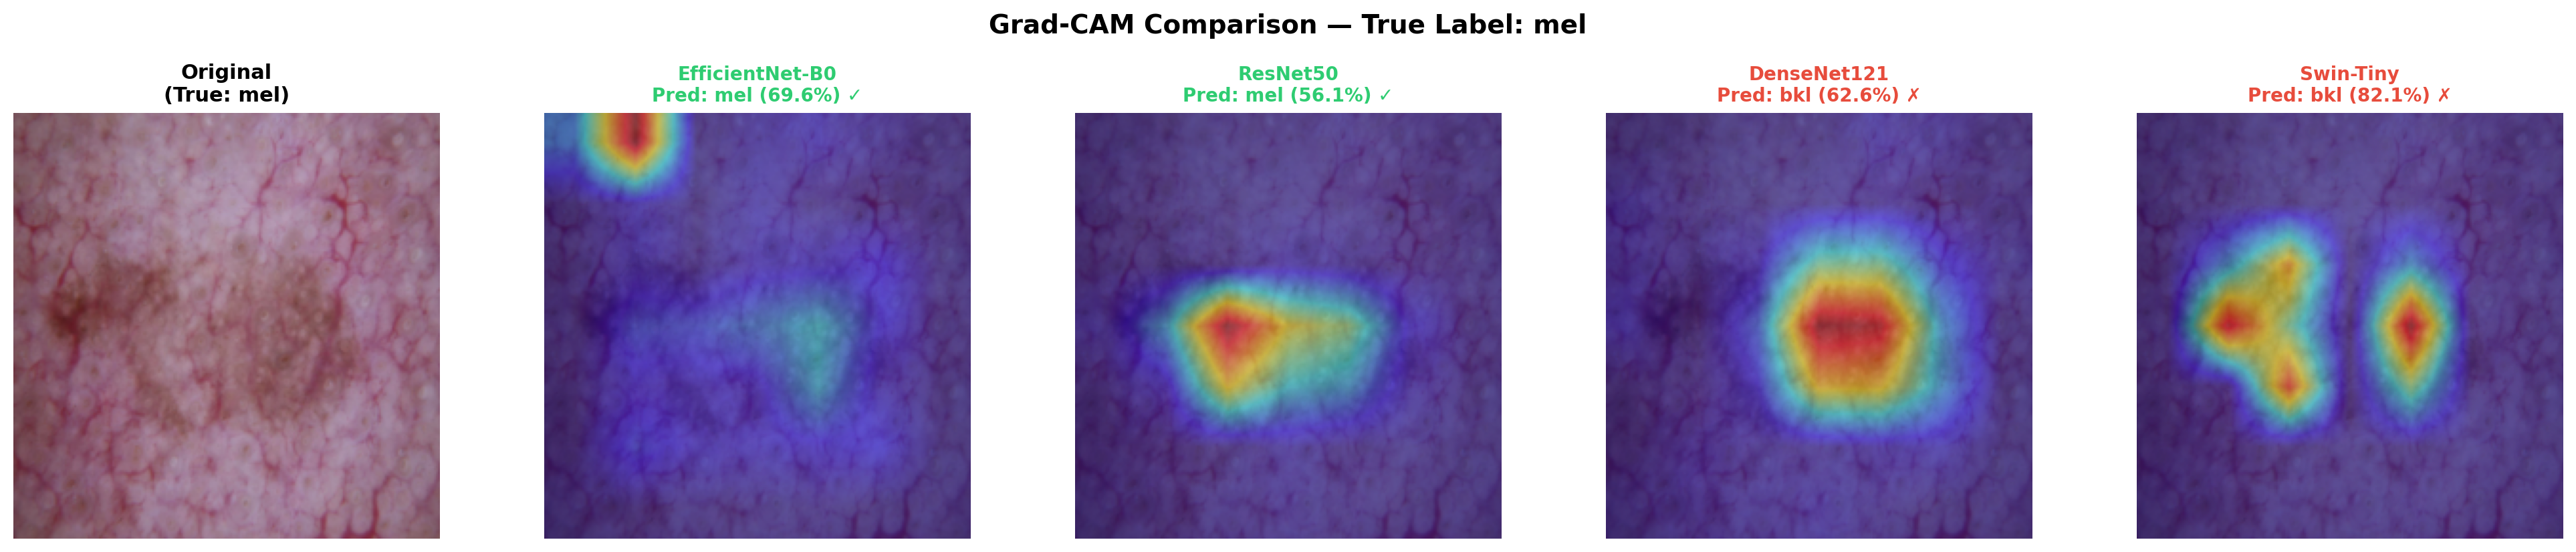
\includegraphics[width=\figwidth]{figures/gradcam_mel_sample.png}
\caption{Grad-CAM cho ảnh melanoma đại diện. Cả bốn mô hình tập trung vào vùng sắc tố bất đối xứng, phù hợp với tiêu chí dermoscopy ABCDE.}
\end{figure}

\section{Nghiên cứu Loại bỏ (Ablation Study)}

\begin{table}[H]
\centering
\caption{Kết quả ablation trên EfficientNet-B0. Mỗi hàng = loại bỏ một thành phần.}
\begin{tabular}{lccccc}
\toprule
\textbf{Cấu hình} & \textbf{Accuracy} & \textbf{Macro F1} & \textbf{AUC} & \textbf{Kappa} & \textbf{$\Delta$ F1}\\
\midrule
Pipeline đầy đủ       & \textbf{0,8836} & \textbf{0,8311} & 0,9522 & \textbf{0,7710} & --- \\
\midrule
$-$ Mixup / CutMix    & 0,8589 & 0,7860 & 0,9486 & 0,7383 & $-$0,0451 \\
$-$ Weighted Sampler   & 0,8762 & 0,8041 & 0,9521 & 0,7487 & $-$0,0270 \\
$-$ Label Smoothing    & 0,8776 & 0,8000 & 0,9674 & 0,7568 & $-$0,0311 \\
$-$ Adv. Augmentation  & 0,8896 & 0,8204 & \textbf{0,9664} & 0,7772 & $-$0,0107 \\
\bottomrule
\end{tabular}
\end{table}

\textbf{Mixup/CutMix} ($-$4,5\% F1): quan trọng nhất --- ngăn ghi nhớ mẫu lớp thiểu số. \textbf{Label Smoothing} ($-$3,1\% F1 nhưng +AUC): đánh đổi giữa ranh giới quyết định và độ sắc nét xác suất. \textbf{Weighted Sampler} ($-$2,7\% F1): ngăn thiên vị NV. \textbf{Advanced Aug} ($-$1,1\% F1 nhưng +Accuracy): chuyển năng lực từ lớp dễ sang lớp khó.

\chapter{Kết luận và Hướng Phát triển}

\section{Tóm tắt Đóng góp}

Khóa luận đã huấn luyện và đánh giá bốn kiến trúc học sâu --- EfficientNet-B0, ResNet50, DenseNet121 và Swin-Tiny --- trên tập ISIC 2018 bảy lớp, với pipeline huấn luyện xây dựng xung quanh tình trạng mất cân bằng 58:1. Bốn thành phần giải quyết mất cân bằng từ các góc độ khác nhau: Lấy mẫu có Trọng số ở mức tải dữ liệu, Mixup và CutMix ở mức tín hiệu huấn luyện, làm mượt nhãn ở mức mục tiêu, và AdamW giảm cosine ở mức tối ưu hóa. Cùng nhau chúng loại bỏ hiện tượng sụp đổ về lớp đa số.

Ở hạt giống đại diện, EfficientNet-B0 (5,3M tham số) vượt ResNet50 (25,6M), DenseNet121 (8M) và Swin-Tiny (28M) trên mọi chỉ số phân loại cứng. Tuy nhiên khi lặp lại thí nghiệm với năm hạt giống ngẫu nhiên, Swin-Tiny mới là mô hình đơn mạnh nhất tính trung bình ($88{,}33 \pm 1{,}96\%$ accuracy so với $87{,}31 \pm 1{,}32\%$ của EfficientNet-B0); xếp hạng ở hạt giống 42 đảo ngược do phương sai của Swin cao hơn. Bài học vẫn giữ: khi dữ liệu hạn chế, hiệu quả kiến trúc và phương pháp huấn luyện quan trọng hơn số tham số, nhưng so sánh một hạt giống không đủ để xếp hạng các kiến trúc gần ngang nhau. Ensemble biểu quyết mềm nâng Macro AUC từ 0,952 lên 0,980 và F1 melanoma từ 0,695 lên 0,744 ở hạt giống đại diện, đồng thời giữ accuracy $89{,}93 \pm 0{,}66\%$ qua năm hạt giống; kiểm định McNemar xác nhận ưu thế ensemble so với mọi mô hình đơn đều có ý nghĩa thống kê ($p < 10^{-7}$ so với mô hình mạnh nhất).

Grad-CAM xác nhận mọi mô hình chú ý đến tổn thương, không phải nhiễu nền. Nguyên mẫu Streamlit tương tác chứng minh các mô hình có thể tích hợp vào giao diện hỗ trợ chẩn đoán chức năng.

Ngoài baseline chỉ-ảnh, hai thí nghiệm mở rộng được thực hiện. Kết hợp metadata bệnh nhân HAM10000 (tuổi, giới, vị trí giải phẫu) qua MLP encoder đẩy ensemble bốn mô hình lên 90,49\% accuracy và 0,873 Macro F1, vượt Pacheco và Krohling (89,0\% / 0,83) và vượt mốc 90\% --- mốc tham chiếu thường được trích dẫn cho phân loại da dựa trên ảnh. Để giới hạn kỳ vọng một cách trung thực, ensemble chỉ-ảnh cũng được đánh giá zero-shot trên PAD-UFES-20 --- 2.298 ảnh smartphone lâm sàng từ modality thu thập khác. Accuracy tụt còn 32,5\%, giảm 56 điểm phần trăm --- nhất quán với báo cáo literature cho transfer dermoscopy-sang-smartphone không adapt. AUC theo lớp vẫn giữ 0,61--0,81, xác nhận mô hình không random trên ảnh smartphone nhưng hiệu năng quyết định cứng cần adapt theo modality hoặc fine-tune để dùng được lâm sàng.

\section{Các Phát hiện Chính}

\textbf{Sự đảo ngược accuracy--AUC:} CNN tạo quyết định cứng sắc nét hơn, Swin-Tiny tạo phân phối xác suất được hiệu chỉnh tốt hơn. Mô hình phù hợp phụ thuộc vào nhiệm vụ lâm sàng: cờ nhị phân cần F1 cao (EfficientNet-B0), danh sách xếp hạng rủi ro cần AUC cao (Swin-Tiny).

\textbf{Label Smoothing:} Loại bỏ đồng thời tăng AUC (+0,015) và giảm F1 ($-$3,1\%). Đánh đổi giữa độ sắc nét hiệu chỉnh và chất lượng ranh giới quyết định.

\textbf{Melanoma vẫn khó nhất:} F1 ensemble chỉ 0,744 --- phản ánh độ khó lâm sàng thực sự trong phân tách ung thư hắc tố sớm khỏi nốt ruồi lành tính.

\section{Hạn chế}

\begin{itemize}
    \item \textbf{Thiên kiến nhân khẩu học của tập dữ liệu.} HAM10000 thu thập chủ yếu ở Áo và Mỹ với dân số đa số Fitzpatrick I--III. Triển khai trên bệnh nhân với tông da đậm hơn (Fitzpatrick IV--VI) nhiều khả năng kém hiệu năng, nhất quán với báo cáo thiên kiến tông da ở các hệ thống dermoscopy thương mại. Khóa luận không bao gồm dữ liệu Việt Nam hoặc dữ liệu địa phương đại diện, nên khoảng cách nhân khẩu học được thừa nhận nhưng chưa được đo lường.
    \item \textbf{Khoảng cách modality thu thập.} Đánh giá ngoài phân phối trên PAD-UFES-20 định lượng mức giảm 56 điểm phần trăm accuracy khi cùng một ensemble chỉ-ảnh chạy trên ảnh smartphone lâm sàng thay vì dermoscopy ánh sáng phân cực. Pipeline chưa triển khai được trên ảnh consumer-grade nếu không có domain adaptation, fine-tune in-domain, hoặc tiền xử lý đặc trị cho modality.
    \item \textbf{Phạm vi closed-set bảy lớp.} Classifier bị buộc gán mọi input vào một trong bảy lớp ISIC. Thực hành lâm sàng có hàng chục loại tổn thương, và bất kỳ input nào ngoài bảy lớp huấn luyện (mụn, sẹo, vùng không phải tổn thương) sẽ bị gán nhầm vào lớp gần nhất. Prototype Streamlit giảm thiểu bằng cảnh báo ngưỡng tin cậy, nhưng một bộ phát hiện open-set hoặc OOD chuyên dụng chưa được triển khai.
    \item \textbf{Độ phân giải cố định $224 \times 224$.} Độ phân giải cao hơn, mà các kiến trúc như EfficientNetV2~\cite{tan2021efficientnetv2} thiết kế để khai thác, có thể khôi phục các đặc trưng phân biệt tinh tế bị mất ở kích thước chuẩn, đặc biệt cho các pattern sắc tố và kết cấu tinh tế trong cụm nhầm lẫn MEL/NV/BKL.
    \item \textbf{Tập kiểm tra lớp hiếm nhỏ.} Test set chỉ có 17 Dermatofibroma và 22 Vascular Lesion. Một phân loại sai bổ sung dịch chuyển F1 các lớp này khoảng 0,06, nên các con số per-class cho lớp hiếm mang phương sai cao và không nên diễn giải quá mức.
    \item \textbf{Kiến trúc Transformer đơn.} Chỉ Swin-Tiny được đánh giá. Các biến thể khác (DeiT~\cite{touvron2021deit}, ConvNeXt~\cite{liu2022convnext}, hoặc Swin lớn hơn) có thể cho trade-off accuracy--AUC khác và đặc tính ensemble khác khi kết hợp với các CNN.
    \item \textbf{Không có xác thực lâm sàng tiến cứu.} Các mô hình chưa được triển khai trong workflow patient-facing hoặc đánh giá bởi bác sĩ da liễu thực hành theo thời gian thực. Các nghiên cứu so sánh human--AI và đánh giá chấp nhận của bác sĩ vẫn là điều kiện tiên quyết cho mọi cân nhắc triển khai.
\end{itemize}

\section{Hướng Phát triển}

\begin{itemize}
    \item \textbf{Domain adaptation cho ảnh lâm sàng.} Mức giảm 56 điểm phần trăm OOD trên PAD-UFES-20 thiết lập một mục tiêu định lượng. Style-transfer preprocessing, adversarial domain adaptation, hoặc fine-tune trên một bộ ảnh smartphone gắn nhãn nhỏ đều được kỳ vọng thu hẹp phần đáng kể khoảng cách đó.
    \item \textbf{Open-set và OOD detection.} Bổ sung một component chuyên dụng (Mahalanobis distance trên features backbone, Energy-based score, hoặc tín hiệu tái cấu trúc autoencoder) sẽ cho phép hệ thống từ chối input không phải tổn thương da, thay vì buộc gán bảy lớp mà người dùng phải tự loại trừ.
    \item \textbf{Augmentation theo tông da và phân tích fairness.} Augmentation hue/saturation theo Fitzpatrick, kết hợp với loss term fairness theo subgroup, sẽ trực tiếp đối phó thiên kiến nhân khẩu học thừa hưởng từ phân phối huấn luyện HAM10000. Khi có dữ liệu Việt Nam hoặc dữ liệu địa phương đại diện, các con số fairness có thể được đo lường.
    \item \textbf{Huấn luyện độ phân giải cao hơn.} Các kiến trúc thiết kế cho input lớn hơn có thể khôi phục features bị mất ở $224 \times 224$, đặc biệt cho cụm nhầm lẫn MEL/NV/BKL nơi các khác biệt texture nhỏ mang thông tin chẩn đoán.
    \item \textbf{Huấn luyện trước tự giám sát.} Các phương pháp như DINO~\cite{caron2021dino} có thể trích xuất biểu diễn thị giác mạnh từ các bộ sưu tập dermoscopy không nhãn lớn trước khi fine-tune trên dữ liệu có nhãn, có khả năng giảm yêu cầu dữ liệu hiệu quả và cải thiện tổng quát hóa lớp thiểu số.
    \item \textbf{Phân loại hỗ trợ phân đoạn.} Dự đoán đồng thời ranh giới tổn thương~\cite{hasan2020dsnet} cùng với nhãn bệnh sẽ cho mô hình giám sát không gian rõ ràng cho các features ranh giới liên quan nhất tới phân biệt melanoma--nevus.
    \item \textbf{Knowledge distillation cho triển khai.} Nén ensemble bốn mô hình thành một mô hình nhẹ duy nhất sẽ giữ phần lớn lợi thế accuracy đồng thời giảm chi phí inference về một forward pass, yêu cầu thực tiễn cho triển khai mobile hoặc point-of-care.
    \item \textbf{Đánh giá lâm sàng tiến cứu.} Một nghiên cứu có kiểm soát so sánh output của hệ thống với một hội đồng bác sĩ da liễu thực hành trên tập case đại diện là bước tiếp theo cần thiết trước khi đưa ra bất kỳ tuyên bố triển khai nào.
\end{itemize}


\end{document}
